\documentclass[final]{fhnwreport}       	%[mode] = draft or final
                                        	%{class} = fhnwreport, article, 
                                        	%          report, book, beamer, standalone
%%---Main Packages-----------------------------------------------------------------------
\usepackage[english, ngerman]{babel}	%Mul­tilin­gual sup­port for LaTeX
\usepackage[T1]{fontenc}				%Stan­dard pack­age for se­lect­ing font en­cod­ings
\usepackage[utf8]{inputenc}				%Ac­cept dif­fer­ent in­put en­cod­ings
\usepackage{lmodern}                    %The newer Font-Set
\usepackage{textcomp}					%LaTeX sup­port for the Text Com­pan­ion fonts
\usepackage{caption}					%Customising captions in floating environments
\usepackage{graphicx} 					%En­hanced sup­port for graph­ics
\usepackage{float}						%Im­proved in­ter­face for float­ing ob­jects
\usepackage{ifdraft}                    %Let you check if the doc is in draft mode
\usepackage{enumitem}


%%---Useful Packages---------------------------------------------------------------------
\usepackage{colortbl}	
\usepackage{color}						%Colour control for LaTeX documents
\usepackage[pdftex,dvipsnames,tabl]{xcolor}  %Driver-in­de­pen­dent color ex­ten­sions for LaTeX
\usepackage{csquotes}                   %Simpler quoting with \enquote{}
\usepackage{siunitx} 					%A com­pre­hen­sive (SI) units pack­age
%\usepackage{listings}					%Type­set source code list­ings us­ing LaTeX
\usepackage[bottom]{footmisc}			%A range of foot­note op­tions
\usepackage{footnote}					%Im­prove on LaTeX's foot­note han­dling
\usepackage{verbatim}					%Reim­ple­men­ta­tion of and ex­ten­sions to LaTeX ver­ba­tim
\usepackage[textsize=footnotesize]{todonotes} %Mark­ing things to do in a LaTeX doc­u­ment
\usepackage{titling}					%Control over the typesetting of the \maketitle command
\usepackage[euler]{textgreek}		%Allows to write greek letters without entering math-mode (\textOmega)

%%---Tikz Packages-----------------------------------------------------------------------
\usepackage{standalone}
\usepackage{tikz}
\usepackage{circuitikz}
\usetikzlibrary{arrows}
\usetikzlibrary{calc}
\usetikzlibrary{intersections}

%%---Math Packages-----------------------------------------------------------------------
\usepackage{amsmath}					%AMS math­e­mat­i­cal fa­cil­i­ties for LaTeX
\usepackage{amssymb}					%Type­set­ting symbols (AMS style)

%\usepackage{amstext}
%\usepackage{amsfonts}
%\usepackage{breqn}
%\usepackage{array}						%Ex­tend­ing the ar­ray and tab­u­lar en­vi­ron­ments
%\usepackage{amsthm}					%Type­set­ting the­o­rems (AMS style)

%%---Table Packages----------------------------------------------------------------------
\usepackage{tabularx}					%Tab­u­lars with ad­justable-width columns
%\usepackage{longtable}
%\usepackage{multirow}					%Create tab­u­lar cells span­ning mul­ti­ple rows
\usepackage{multicol}					%In­ter­mix sin­gle and mul­ti­ple columns



%%---PDF / Figure Packages---------------------------------------------------------------
\usepackage{pdfpages}					%In­clude PDF doc­u­ments in LaTeX
%\usepackage{pdflscape}					%Make land­scape pages dis­play as land­scape
%\usepackage{subfig}					    %Fig­ures di­vided into sub­fig­ures

%%---Other Packages----------------------------------------------------------------------
%\usepackage{xargs}                     %De­fine com­mands with many op­tional ar­gu­ments


%%---Bibliography------------------------------------------------------------------------
\usepackage[style=ieee,urldate=comp,backend=biber]{biblatex}
\addbibresource{literature/bibliography.bib}

%%---Main Settings-----------------------------------------------------------------------
\graphicspath{{./graphics/}}			%Defines the graphicspath
\geometry{twoside=false}				    %twoside=false disables the "bookstyle"
\setlength{\marginparwidth}{2cm}
\overfullrule=5em						%Creates a black rule if text goes over the margins => debugging




%%---User Definitions--------------------------------------------------------------------
%%Tabel-Definitions: (requires \usepackage{tabularx})
\newcolumntype{L}[1]{>{\raggedright\arraybackslash}p{#1}}    %column-width and alignment
\newcolumntype{C}[1]{>{\centering\arraybackslash}p{#1}}
\newcolumntype{R}[1]{>{\raggedleft\arraybackslash}p{#1}}
\usepackage{subcaption}


%%---Optional Package Settings-----------------------------------------------------------
%Listings-Settings: (requires \usepackage{listings}) => Example with Matlab Code
%\lstset{language=Matlab,%
%    basicstyle=\footnotesize\ttfamily,
%    breaklines=false,%
%    morekeywords={switch, case, otherwise},
 %   keywordstyle=\color{Blue},%
 %  tabsize=2,
    %morekeywords=[2]{1}, keywordstyle=[2]{\color{black}},
%    identifierstyle=\color{Black},%
%    stringstyle=\color{Purple},
%    commentstyle=\color{Green},%
%    showstringspaces=false,%without this there will be a symbol in the places where there is a space
%    numbers=left,%
%    numberstyle={\tiny \color{black}},% size of the numbers
%    numbersep=9pt, % this defines how far the numbers are from the text
    %emph=[1]{word1, word2,...},emphstyle=[1]\color{red}
%}							

%Hurenkinder und Schusterjungen verhindern (kein Scherz, Google es)
\clubpenalty10000
\widowpenalty10000
\displaywidowpenalty=10000	



%Titel mit Mathematik immer fett drucken
\usepackage{sectsty}
\allsectionsfont{\boldmath}



			               	%loads all packages, definitions and settings											
\title{Fachbericht}  		        		%Project Title
\author{Team Schenk \& Aebi}      				    %Document Type => Technical Report, ...
\date{\today}          				   	%Place and Date

\begin{document}

%%---TITLEPAGE---------------------------------------------------------------------------------
\thispagestyle{empty}
%	\ohead{\includegraphics[scale=0.5]{Bilder/Logo_FHNW.jpg}}
	\begin{figure}
		 \vspace*{-\topskip}\vspace*{-\headsep}
		
\includegraphics[scale=1]{graphics/fhnw_ht_logo_de.pdf}
	\end{figure}
	\begin{center}
		\vspace*{2cm}
		{\huge{\textbf{\thetitle}}}\\
		\vspace*{0.5cm}
		
		{\scshape\Large Projekt 5 Cocktailmaschine - \theauthor \\} \Large{\today}
		\vfill
		\begin{normalsize}
			{\begin{tabbing}
					\textbf{Betreuender Dozent:} \hspace{5cm}\= Prof. Dr. Schleuniger, Pascal\\[0.8cm]		
					\textbf{Team:} \>Schenk, Kim \\ \>Aebi, Robin\\[0.8cm]
					\textbf{Studiengang:} \>Elektro- und Informationstechnik
					\\[0.8cm]	\textbf{Semester:} \>Herbstsemester 2019
			\end{tabbing}}
		\end{normalsize}
		\vfill
	\end{center}
\clearpage
			
%%---ABSTRACT----------------------------------------------------------------------------
\selectlanguage{english}				%ngerman or english
\thispagestyle{empty}
\paragraph{Danksagung}\mbox{}

Da diese Arbeit zur Zeit des Corona bedingten Lockdowns entstanden ist und keine Möglichkeit bestand in den Schulwerkstätten zu arbeiten, konnte nicht auf externe Hilfe verzichtet werden. Vor allem auch weil die Arbeit ein voll umfängliches Produkt darstellt, welches nicht nur elektrotechnische sondern auch mechanische Komponenten beinhaltet wurde eine gesamte Werkstatt benötigt. Diese wurde und von Claudia und Thomas Aebi zur Verfügung gestellt. Weiter wurden einige mechanische Komponenten auf der Drehbank angefertigt, was spezielles Equipment voraus setzte. Dabei wurden wir von Peter Aebi fachkräftig unterstützt. Im weiteren konnten wir uns jeder Zeit auf Herrn Christoph Biel verlassen, welcher die Studenten mit viel Herzblut jeder Zeit unterstützt. Sei es wenn man Messgeräte benötigt, Bestellungen erfassen oder Geld zurückfordern muss. Zu guter Letzt wurden wir durch das ganze Projekt hindurch von unserem Fachcoach Herrn Schleuniger unterstützt. Bei all diesen Personen wollen wir uns herzlichst bedanken. Ohne diese Mithilfe wäre es uns nicht möglich gewesen dieses Projekt auf diese Weise zu vollenden.     

\newpage




\begin{abstract}

Der technologische Fortschritt ist seit Jahren am explodieren. Das Internet der Dinge, oder auf Englisch auch Internet of things, kurz IoT, ist ein Produkt aus diesem Fortschritt. Es beschreibt ein Netz aus physikalischen und virtuellen Komponenten, welche miteinander kommunizieren, um einem Grösseren ganzen zu dienen. Im Zentrum steht nebst der Interaktion zwischen Mensch und elektronischen Systemen die Interaktion zwischen verschiedenen Systemen. In dieser Bachelorthesis wird anhand der Entwicklung einer IoT-Cocktailmaschine demonstriert, welche Teilsysteme wie genutzt werden können, um ein fertiges Produkt zu entwickeln.
Die Herausforderung liegt im gesamten Produktentwicklungsprozess und umfasst:\\

\begin{itemize}
\item die Projektauswahl, -Planung und -Abgrenzung
\item das Erstellen der Anforderungen an das Gesamtsystem und der darin enthaltenen Teilsysteme
\item die Wahl, das Testen, Implementieren der Komponenten
\item die Evaluation des Gesamtsystems
\end{itemize}
\mbox{}\\

Für die Umsetzung benötigt es einen Software- , einen elektronischen und einen mechanischen Teil.
Der mechanische Teil beinhaltet die Unterbringung der Zutaten und der Elektronik, der Beförderung und Messung der Flüssigkeiten mittels Pumpen und Durchflusssensoren sowie die Bewegung des Glases mit einem bürstenlosen Gleichstrommotor. Die Verschalung rundet die Maschine ab und verhindert, dass sensible Teile angefasst oder nass werden können.
Zum elektrotechnischen Teil gehört unter anderem ein Display, über welches der Benutzer die Cocktails auswählen, erstellen oder bearbeiten kann. Eine mikroSD-Karte ermöglicht Cocktails, Zutaten und maschinenspezifische Zustände zu speichern. Ein RFID-Reader liest Tags aus, was es ermöglicht Lieblingsgetränke zu hinterlegen und direkt in der Maschine anzuwählen.
Für die Verbindung zwischen Android-Applikation und Cocktailmaschine wird ein Wireless-/Bluetoothmodul verwendet. Mittels MOSFET-Schaltungen werden während der Erstellung von Cocktails die Pumpen vom Mikrocontroller ein- und ausgeschaltet. Die Ansteuerung und Regelung des bürstenlosen Gleichstrommotors ergibt sich aus einem FOC-Treiber und einem Gate-Treiber. Der ABN-Encoder liefert das Feedback zur Lage des Rotors, welches benötigt wird als Regelparameter für den FOC-Treiber.
Die entwickelte Leiterplatine gehört zum Elektronikteil und bildet das Bindeglied zwischen Mechanik und Elektronik.
Der Softwareteil wird in vier Teilsoftwares geteilt. Alle Teile werden in verschiedenen Sprachen geschrieben. Die Firmware auf dem Mikrocontroller, welche in C geschrieben wurde, regelt den Programmfluss der gesamten Maschine. Die Firmware auf dem Wireless-/Bluetoothmodul, welche in Arduino geschrieben wurde, bildet die Schnittstelle zwischen den Signalen der Android-Applikation und der Firmware. Die Android-Applikation wurde mit dem Online-Tool App-Inventor entwickelt und ermöglicht dem Anwender Cocktails über Fernzugriff zu erstellen und einem RFID-Tag zu zu weisen. Bei der letzten Programmierumgebung handelt es scih um den Nextion Editor, mit welchem Nextion Displays Programmiert werden können.


Damit alle Komponenten ansteuerbar sind, mussten einige Anpassungen an der Hardware vorgenommen werden. Dazu gehören aufgrund von Störungen auf dem SPI-Bus das Umlegen der SPI-Leitungen des RFID-Readers vom Mikrocontroller auf das Wireless-/Bluetoothmodul und das Umlegen der SPI-Leitungen des FOC-Treibers auf ein separates Software-SPI. Die Motorengruppe läuft aufgrund von Defekten auf der Leiterplatine mit externen Boards. Die Firmware läuft bis auf wenige Punkte sauber. Dazu gehört zum Beispiel, dass der Abbruchprozess beim Erstellen eines Getränkes nicht wunschgemäss Funktioniert. Die gesetzten Ziele wurden alle erreicht werden. Ausserdem wurden fast alle Pflichtziele erfüllt.





%Die in dieser Bachelorthesis entwickelte Cocktailmaschine ist ein IoT\footnote{\textbf{I}nternet \textbf{o}f \textbf{T}hings}-Produkt. Die Elemente sind eingebettet in Sensoren, Software und andere Technologien, welche es erlauben mit anderen Geräten zu kommunizieren. Zu den Elementen gehören ein Mikrocontroller mit zugehöriger Programmierschnittstelle, zwölf Pumpen sowie zugehörige Durchflusssensoren, ein RFID-Transponder, ein WiFi/Bluetooth-Modul mit zugehöriger Programmierschnittstelle, eine SD-Karte, ein FOC-Motorentreiber mit zugehörigem Kraft-Teil, ein Display und eine RGBW-LED-Regelung. Anhand der ersten Erfahrungen im Projekt 5 wurde eine Leiterplatine gelayoutet, welche die erwähnten Elemente verbindet. Über eine Android-Applikation wird den Benutzern die Möglichkeit geboten, einen neuen Cocktail zu erstellen oder das Lieblingsgetränk auszuwählen. Das gewählte Getränk kann dann vor Ort über den RFID-Tag bestellt werden. Die Mechanik besteht aus einem Aluminiumgerüst, welches verschalt wurde. Zusätzlich wurde zur Kühlhaltung eine Styroporbox um die Zutaten gebaut. Ein durch einen Motor angetriebener Schlitten fährt das Glas unter den gewünschten Flüssigkeitsauslass, wo das Glas befüllt wird. Die Dokumentation enthält eine Beschreibung der Platine und der darauf befindenden Elementen, eine Anleitung zur Inbetriebnahme der Elemente und einen Software-Teil. Das Produkt wurde physikalisch abgegeben und ist voll funktionsfähig.

\end{abstract}


%%---TABLE OF CONTENTS-------------------------------------------------------------------
\pagenumbering{Roman}		
\selectlanguage{ngerman}				%ngerman or english
\tableofcontents
\clearpage

%%---TEXT--------------------------------------------------------------------------------
\pagenumbering{arabic}
\clearpage
\section{Einleitung}
\label{sec:Einleitung}

Eine gelungene Party auf die Beine zu stellen verlangt einem einiges ab. Vor allem kostet es eine Menge Aufwand und Zeit. Dies gilt besonders, wenn es darum geht mit vielen Freunden zusammen zu feiern. Neben der gelungenen Musikauswahl und den Snacks darf eines auf gar keinen Fall fehlen, die Getränke. Um diese sicherzustellen, gibt es mehrere Möglichkeiten. Einerseits könnte jeder seine eigenen Getränke mitbringen, was jedoch bedeutet, dass es unter Umständen eine riesige Sauerei gibt oder viele Flaschen in der Gegend rumstehen. Anderseits könnte man als Gastgeber selber anbieten Cocktails zu mixen und so den Getränkenachschub zu gewährleisten. Da gibt es jedoch ein grosses Problem. Denn wären wir die Gastgeber, so würden wir nicht den ganzen Abend hinter der Bar stehen wollen, sondern lieber bedenkenlos mitfeiern. Damit genau dies möglich ist haben wir uns in diesem und dem nächsten Projekt (5\&6) dazu entschieden eine automatisierte Cocktailmaschine zu entwerfen. Diese soll vollkommen autonom arbeiten und sollte problemlos von jeder beliebigen Person und in fast jedem Zustand bedient werden können. 

In den folgenden Kapiteln ist dokumentiert, wie die Cocktailmaschine aussehen soll und aus welchen Teilsystemen diese bestehen wird. Ausserdem werden die einzelnen Teilsysteme genauer unter die Lupe genommen und in einem systemspezifischen Testverfahren evaluiert. Dieses Projekt bietet demnach die Basis des Projekt 6 und soll dieses so gut wie möglich vorbereiten.

\pagebreak
\section{Ausgangslage}
\label{sec:Ausgangslage}

Die Basis für das Projekt 6 hat das Projekt 5 gebildet, in welchem ein Konzept erstellt wurde, welches die Hauptkomponenten der Maschine festlegte und deren Arbeitsweise. Aus dieser Entscheidungsfindung wurde dann ein Blockschaltbild erstellt, welches in Abbildung \ref{fig:P5_Blockschaltbild_Partymixer} zu sehen ist. Ein weiterer Teil des Projekt 5 war es, die gewählten Komponenten und die daraus entstandenen Teilsysteme in einem Testaufbau aufzubauen und zu evaluieren. Dazu gehörten die Speisungen (48V, 12V, 5V und 3.3V), der Mikrocontroller, das Display, der Motor, die Pumpenansteuerung und die Durchflussmessgeräte.

\begin{figure}[H]
\center
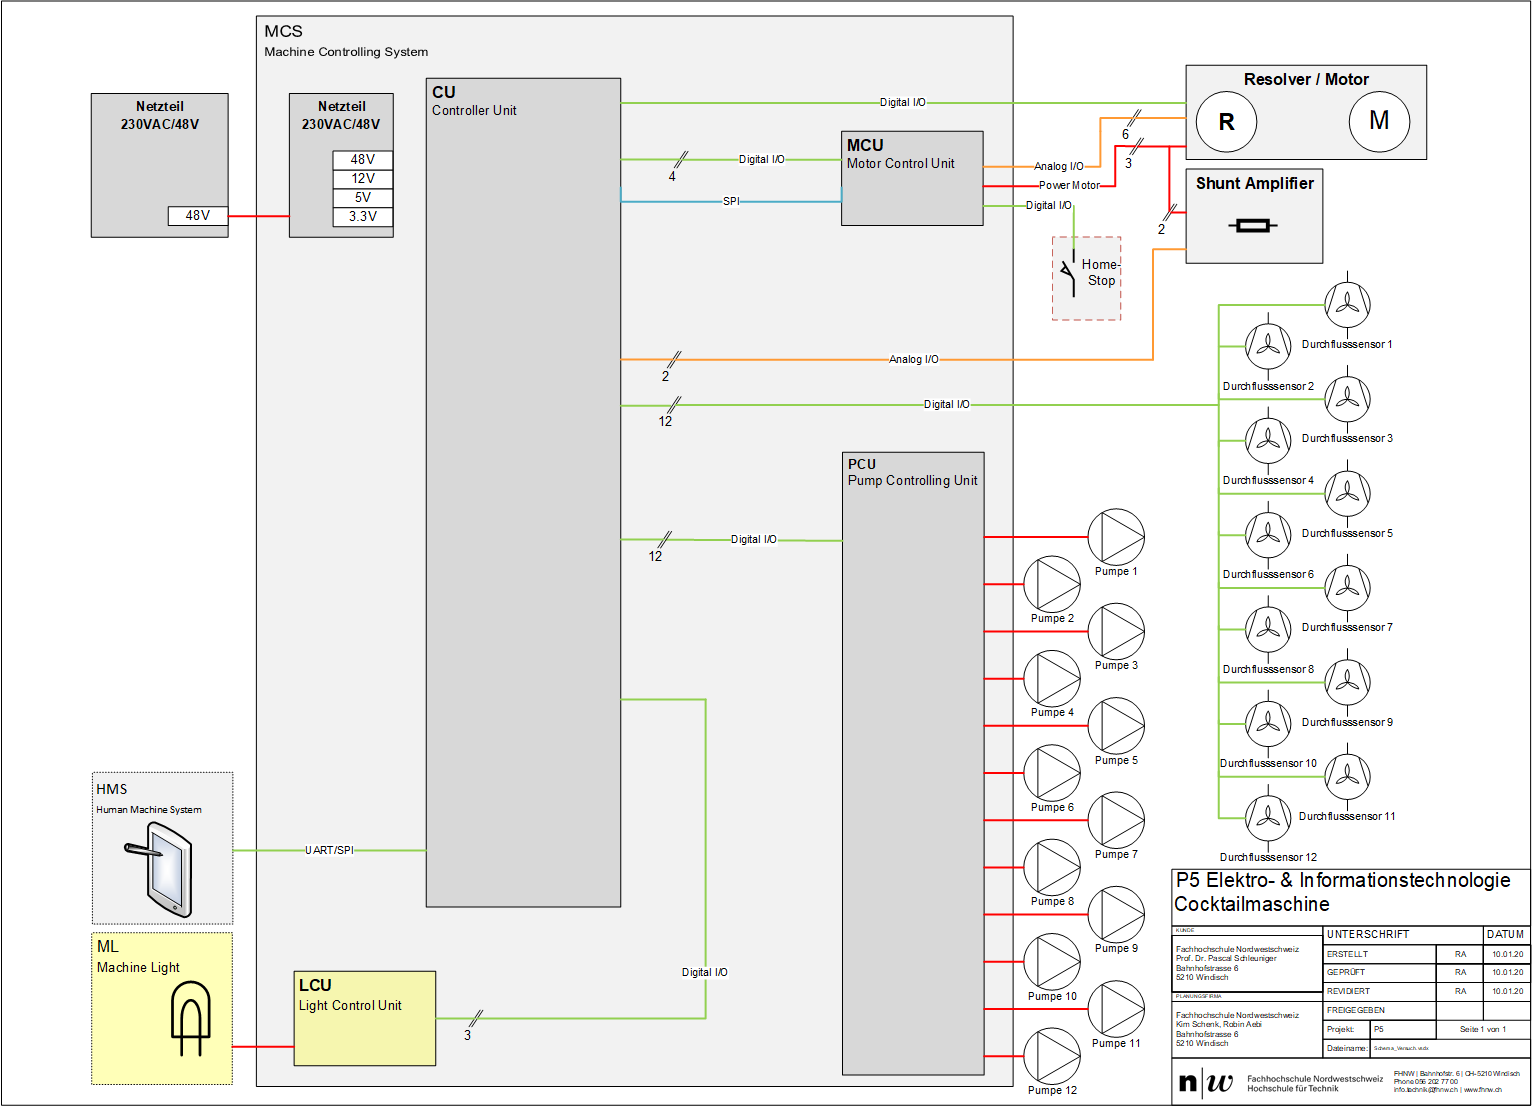
\includegraphics[angle=90, width = 0.82\textwidth]{graphics/P5-Blockschema}
\caption{Blockschaltbild des PartyMixer's gemäss Projekt 5.}
\label{fig:P5_Blockschaltbild_Partymixer}
\end{figure}

\newpage



\subsection{Blockschaltbild}
\label{subsec:Blockschaldbild}



\subsection{Komponentenauswahl}
\label{subsec:Komponentenauswahl}

Um die Anforderungen gemäss Blockschaltbild erfüllen zu können sind neue Komponenten implementiert worden. Diese sollen nun genauer unter die Lupe genommen werden.

Speisungen: 
\begin{itemize}
\item Sorgen für die notwendigen Betriebsspannungen
\end{itemize}

Mikrocontroller: 
\begin{itemize}
\item Sorgen für die notwendigen Betriebsspannungen
\end{itemize}



\newpage

\section{Neue Hardware}
\label{sec:Neue Hardware}

Im folgenden Kapitel werden die Hardware-Teile beschrieben, welche im Projekt 5 noch nicht erarbeitet wurden. Zuerst werden grundlegende Anforderungen und Inhalte beschrieben, welche zur Auswahl der Bauteile feführt hat.

\subsection{USB-B}
\label{subsec:USB-B}

Auf der Leiterplatte gibt es zwei Komponenten, die programmiert werden müssen. Der Mikrocontroller und das WiFi-Modul. Beide werden über die UART-Schnittstelle 0 programmiert. Um diese zu programmieren braucht es eine entsprechende Schnittstelle, welche mit einer USB-B-Schnittstelle realisiert wird.

Die USB-B-Schnittstelle benötigt jedoch nur zwei Kommunikationsleitungen (D+ und D-). Deswegen benötigt es einen USB-UART-Converter. Hier wurde auf das Flash-Interface von Arduino zurückgegriffen \cite{arduino_cc_arduino_2017}, um die Schaltung für den Mikrocontroller zu planen und auf das Flash-Interface des ESP32 \cite{espressif_systems_esp32_2016}, um die Schaltung für den ESP32 zu planen. Darin ist ersichtlich, dass für den Mikrocontroller und ESP folgende Leitungen nötig sind:

\begin{itemize}
\item Mikrocontroller
\begin{itemize}
\item RX ==> TX
\item TX ==> RX
\item Reset ==> über Kondensator an DTR
\end{itemize}
\item ESP32
\begin{itemize}
\item RX ==> TX
\item TX ==> RX
\item EN ==> über Schaltung an DTR
\item IO\_0 ==> über Schaltung an RTS
\item IO\_13 ==> über Widerstand an RTS
\item IO\_15 ==> über Widerstand an CTS
\end{itemize}
\end{itemize}

Auch hier wurde vom Arduino Uno-Board abgekpufert und der selbe Chip verwendet, um die USB-Signale in UART-Signale zu konvertieren. Das vorkommende Bauteil ist der CP2102N. Da dieser Chip ein TQFP-28-Gehause hat, könnte es auch schwierigkeiten geben beim Löten. Deswegen wird auch ein Breakout-Board (BOB) mitgeplant, damit es eine Ausweichmöglickeit gibt falls die Bauteile zu klein sind. Dabei ist zu achten, dass das BOB genügend Ausgangspins hat, speziell beim ESP32.

\begin{figure}[!h]
\center
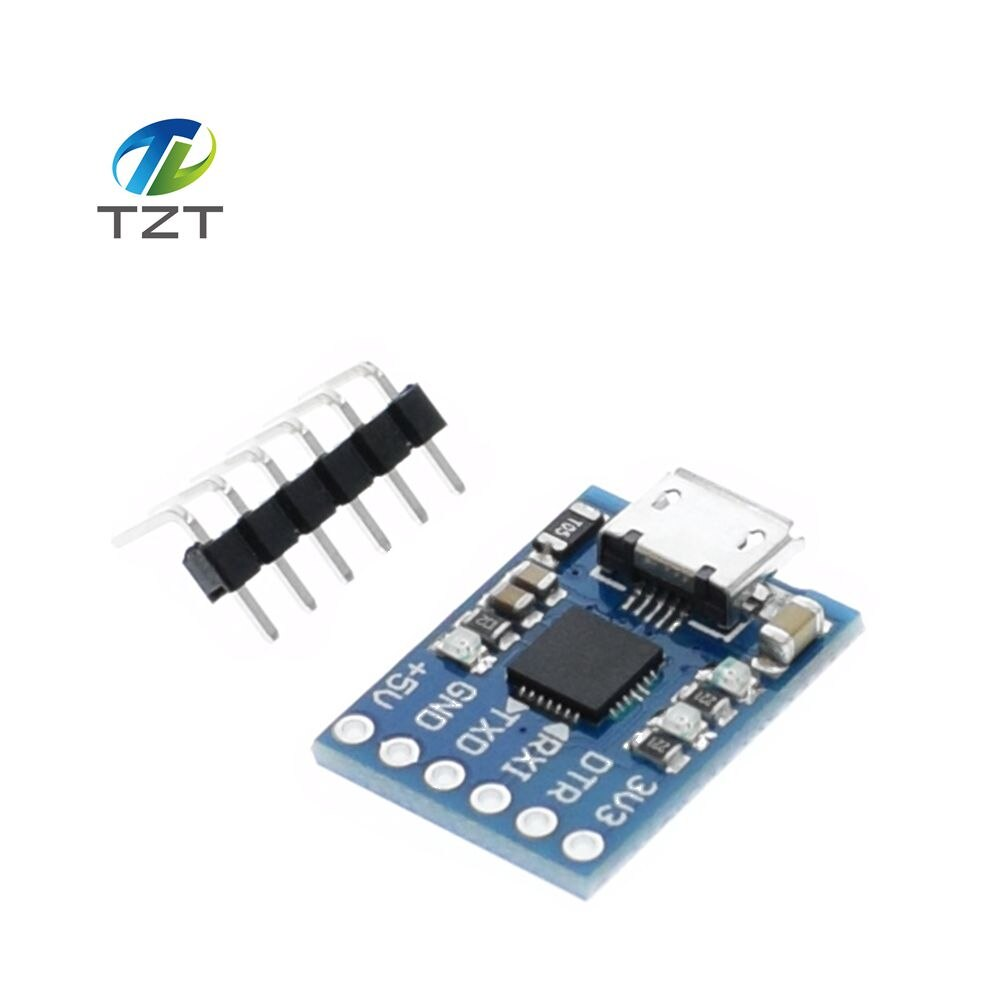
\includegraphics[width = 0.5\textwidth]{graphics/Produktbild_USB_UART_uC}
\caption{CP2102N-BOB für uC.}
\label{fig:Produktbild_USB_UART_uC}
\end{figure}

\begin{figure}[!h]
\center
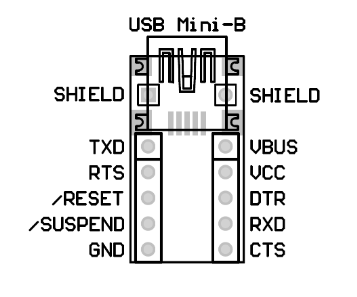
\includegraphics[width = 0.5\textwidth]{graphics/Produktbild_USB_UART_ESP}
\caption{CP2102N-BOB für ESP.}
\label{fig:Produktbild_USB_UART_ESP}
\end{figure}

\subsection{Wirelessmodul}
\label{subsec:Wirelessmodul}


		
\subsection{RFID}
\label{subsec:RFID}

Eine vorgesehene Funktion der Maschine ist, dass der User ohne Suchen sein Lieblingsgetränk zubereiten lassen kann. Dafür wird auf ein System zurückgegriffen, was öfters für Zutrittskontrollen oder Ähnliches verwendet wird. Nämlich RFID \footnote{Radio Frequency IDentification}.

Um schnell ein funktionierendes Teilsystem testen zu können, soll ein Breakout-Board verwendet werden. Eine Recherche hat ergeben, dass es nicht allzu viele Produkte gibt. Ein Eingenzungskriterium war, dass es es für den Ausgewählten IC eine vorgeschriebene Library gibt, welche sich mit Arduino bewährt hat. Der Chip, welcher diese Anforderungen erfüllt, ist der \textbf{Mifare MFRC522}. Er ist in Abbildung \ref{fig:Produktbild_RFID_MFRC522} abgebidet. Dieses Brakeout-Board kann ausserdem an der Verschalung der Maschine angeschraubt werden. Somit kann er sich an einer Stelle befinden, welche weiter weg von der Hauptsplatine ist.
Das Modul arbeitet auf 13.56MHz und gilt somit als kurzwelliges System (HF).

Der MFRC522 ist der Reader im RFID-System. Er kann Daten lesen und ggf. auch schreiben. Er erzeugt ein hochfrequentes, elektromagnetisches Wechselsignal mit einer Frequenz von 13.56MHz. Der RFID-Tag wird von der Energie des Wechselsignals gespiesen. Durch Kurzschliessen der Tag-Antenne wird ein Teil der Energie des vom Reader ausgehenden Wechselfeldes verbraucht. Diese Energiedifferenz kann ein Reader detektieren. Die Reichweite für ein solches System beträgt weniger als 10cm.

Alternativ könnte ein Tag mit einer Batterie gespiesen werden. Somit erhöht sich die Reichweite des Readers, die Latenzzeiten werden kürzer und der Anwendungsbereich würde grösser.

%\begin{figure}[!h]
%\center
%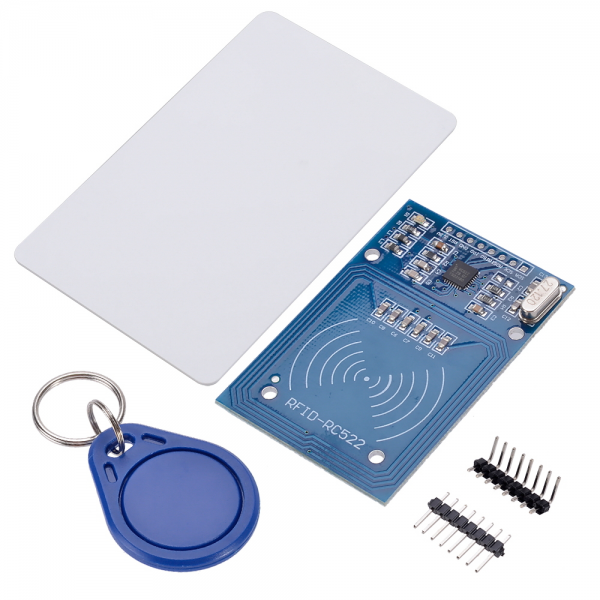
\includegraphics[width = 0.6\textwidth]{graphics/Produktbild_RFID_MFRC522}
%\caption{MFRC522.}
%\label{fig:Produktbild_RFID_MFRC522}
%\end{figure}



\newpage
\subsection{Beleuchtung}
\label{subsec:Beleuchtung}

Damit die Maschine optisch etwas hergibt, wurde entschieden die ganze Maschinerie mit LED-Streifen zu verzieren. Dazu ist einerseits das LED-Band von nöten und die geeignete Ansterung dazu. Für die Cocktailmaschine wurde festgelegt, dass der LED-Streifen die benötigten Wirderstände für die LED's schon aufgeklebt hat und die Ansteuerung folglich direkt über FET's geschehen kann. Der Aufbau ähnelt dann dem in Abbildung \ref{fig:LED1} gezeigten Schaltung. Der Streifen wäre Rot eingerahmt, die LED's und Widerstände befinden sich auf dem Band und die zu sehenden Fähnchen für R, G, B und W führen zum Mikrocontroller. Es können auch mehrere Bänder parallel geschaltet werden, wie auf dem Bild.

\begin{figure}[h!]
\center
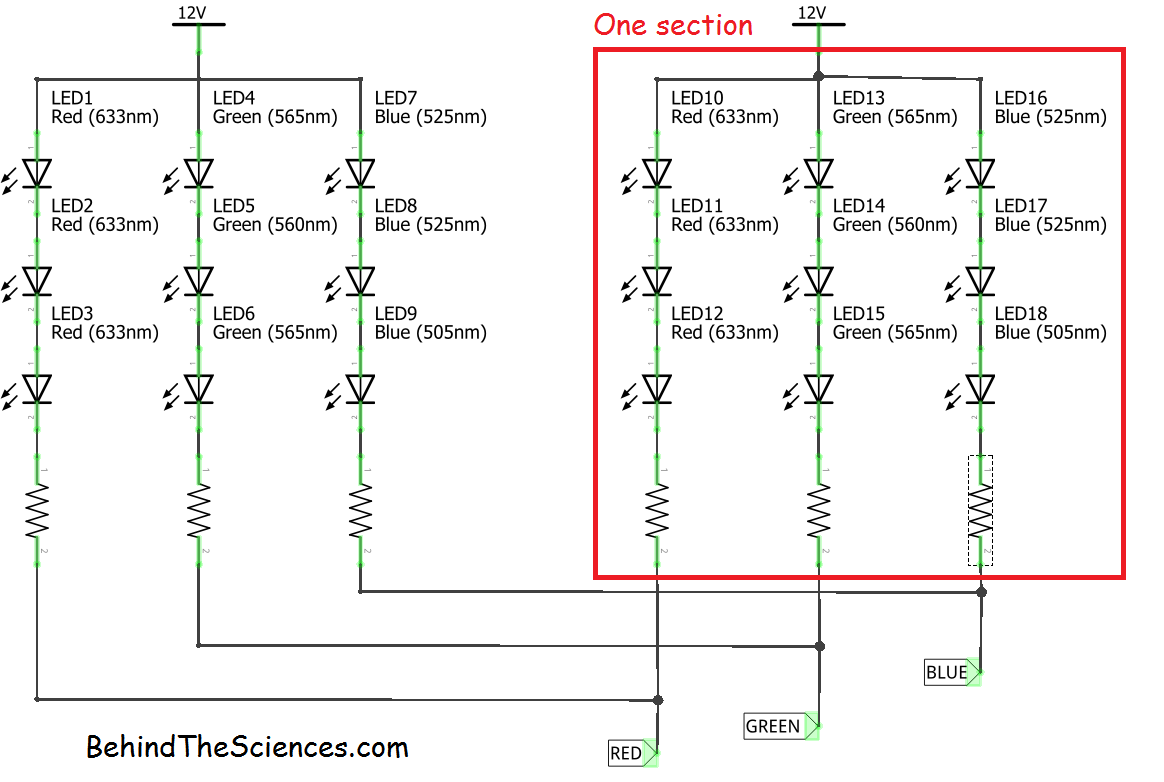
\includegraphics[width = 0.6\textwidth]{graphics/Schema_LED1}
\caption{LED Beispiel.}
\label{fig:LED1}
\end{figure}

\section{Printaufbau}
\label{sec:Printaufbau}



\newpage
\section{Teilsysteme}
\label{sec:Teilsysteme}

Da der Partymixer aus vielen kleineren und grösseren Teilsystemen besteht, werden diese in diesem Kapitel einzeln aufgelistet und im Detail angeschaut.
Es wird dabei bei jedem Teilsystem auf drei Punkte eingegangen, die Problemstellung (Was ist der Zweck der Teilschaltung und wesshalb wird sie benötigt?), das Schema und der Funktionsbeschrieb der Schaltung. Das komplette Schema kann in  \textcolor{red}{\textbf{Anhang Schema}} begutachtet werden.

\todo{Schema richtig Referenzieren und in Anhang machen}

\subsection{Speisungen}
\label{subsec:Speisungen}

Die Speisung, welche das System mit Strom versorgt, ist ein essentieller Bestandteil des PartyMixer's. Im System befinden sich vier verschiedene Speisungen auf verschiedenen Spannungsniveaus. Die Eingangsspannung, womit zwei andere Speisespannungen erzeugt werden und der Motor betrieben wird, wird von einem 48V Netzteil erzeugt. Mittels Step-Down Reglern wird aus der 48V Eingangsspannung eine 12V und eine 5V Speisung erzeugt. Bei der vierten Speisung handelt es sich um einen einfachen Linearregler, welcher aus den 5V eine 3.3V Speisung realisiert. In den folgenden Unterkapitel können die Details der einzelnen Spannungsquellen entnommen werden und deren Aufgabengebiet. Die Grundlage sämtlicher Berechnungen der 5V und 12V Speisungen sind dem Datenblatt entnommen \cite[S.10]{monolithic_power_systems_mp24943_2011}.

\subsubsection{48V Speisung}
\label{subsubec:48V Speisung}

\paragraph{Problemstellung}\mbox{}\\

Der Motor wird mit einer Spannung von 48V betrieben. Dies ist zugleich auch die höchste verwendete Speisespannung. Um diese Speisung gewährleisten zu können, wird ein fertiges Netzteil gemäss  \textcolor{red}{\textbf{Fachbericht 5}} eingesetzt.

\paragraph{Schema}\mbox{}\\

Es wurde im Projekt 5 entschieden, dass die 48V Speisung extern als fertiges Netzteil eingekauft wird. Somit entfällt das Schema für diesen Speisungsteil.  

\begin{figure}[h!]
	\centering
	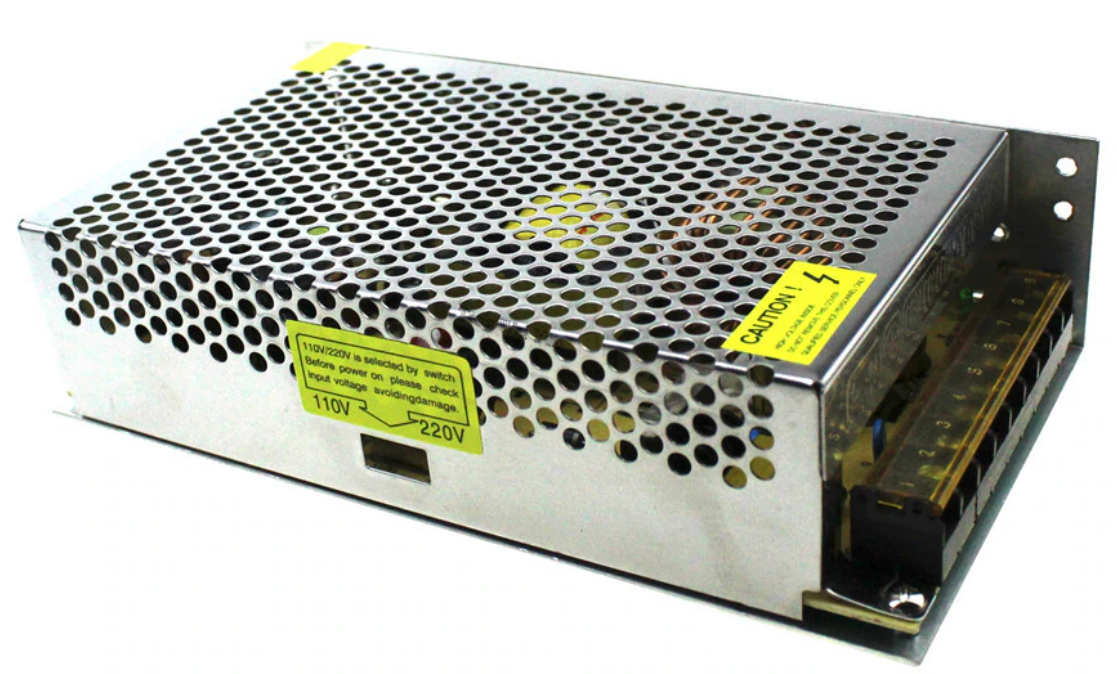
\includegraphics[width=0.8\textwidth]{graphics/Netzteil_48V.png}
	\caption{Anschauungsbild des 48V Netzteils}
	\label{fig:Netzteil_48V}
\end{figure} 


\paragraph{Funktionsbeschrieb}\mbox{}\\

Es musste jedoch unbedingt eine Leistungsabschätzung gemacht werden. Auch diese wurde im Projekt 5 durchgeführt. Unter Berücksichtigung der Schaltungsteile welche noch im Projekt 6 ergänzt werden, wurde dieses dann ausgewählt und eingekauft. Die Leistungsabschätzung kann im \textcolor{red}{\textbf{Fachbericht 5}} eingesehen werden. 

\subsubsection{12V Speisung}
\label{subsubsec:12V Speisung}

Die Pumpen werden mit 12V betrieben, was zur folge hat, dass eine 12V Speisung implementiert werden musste. Dazu wird ein Schaltspannungsregler verwendet. Dieser wandelt mittels Step-Down Prinzip die 48V des Netzteils in eine Konstantspannungsquelle von 12V. Es handelt sich hierbei um einen Regler von Monolithic Power Systems. Genauer gesagt um den MP24943DN-LF. Die Auswahl ist auf dieses Bauteil gefallen, da mit 48V eine relativ hohe Eingangsspannung verarbeitet werden muss. Der MP24943DN-LF kann am Eingang mit Spannungen von 4.5-55V arbeiten und dabei eine Ausgangsspannung von 0.8-45V erzeugen. Dies bei einem maximalen Strom von bis zu 3A. Die Realisierung der 12V Speisung kann in Abbildung \ref{fig:Schema_Speisung_12V} betrachtet werden.\\

\paragraph{Schema}\mbox{}\\

Das Schema in Abbildung \ref{fig:Schema_Speisung_12V} kann in fünf Teile unterteilt werden. Da wäre zuerst der Eingangsfilter, welcher mit C32, C34 \& C36 realisiert ist. Dieser Eingangsfilter wird gefolgt von einem Spannungsteiler, welcher den Enable auf aktiv setzt. Der eigentliche Regler wird mittels des IC7, D6 \& L3 realisiert. Mittels zweier Spannungsteiler, wird die gewünschte Ausgangsspannung, sowie die "Overvoltage-Protection" eingestellt. Vor dem Ausgang der Schaltung ist dann erneut eine Filterstufe implementiert, welche das Ausgangssignal glättet.

\begin{figure}[h!]
	\centering
	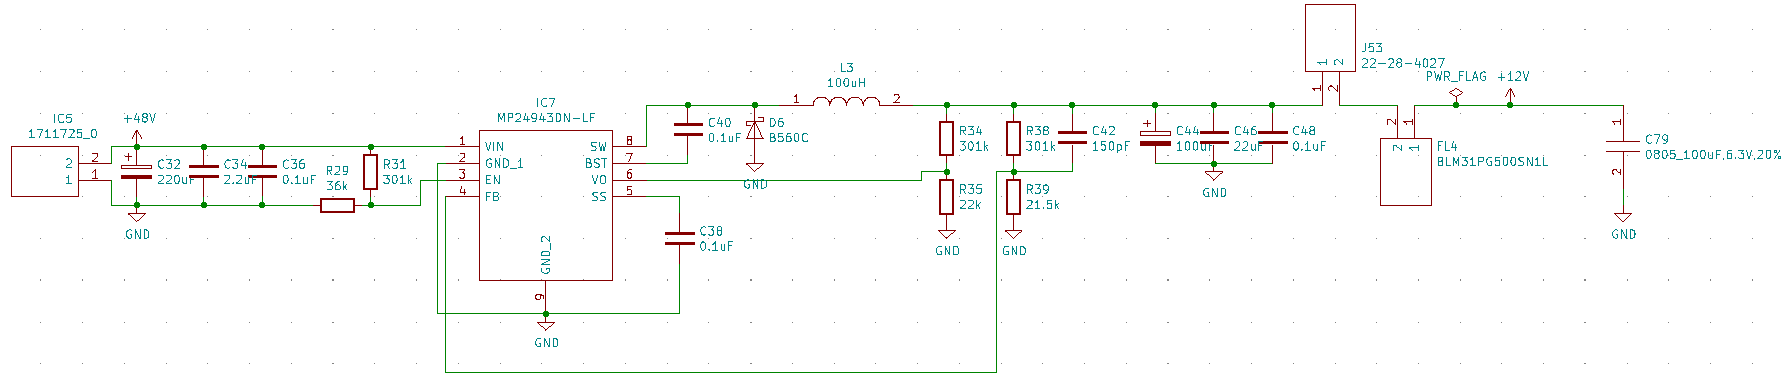
\includegraphics[width=\textwidth]{graphics/Schema_Speisung_12V.png}
	\caption{Schema der 12V Speisung}
	\label{fig:Schema_Speisung_12V}
\end{figure} 

\paragraph{Funktionsbeschrieb der Schaltung}\mbox{}\\

Um den MP24943DN-LF auf aktiv zu setzen, wird eine minimale Spannung von 1.8V vorausgesetzt. Fällt diese unter 0.4V, so wird dieser auf inaktiv gesetzt. Damit der Spannungsregler immer eingeschaltet ist, wird mittels zweier Widerstände R29 \& R31 ein Spannungsteiler realisiert, welcher den Enable (EN) Pin auf 5V und somit auf aktiv setzt. Dieser Spannungsteiler musste implementiert werden, da alle Eingangspins ausser dem V$_{in}$ einen maximale Eingangspegel von 6.5V verkraften können.

Die gewünschte Ausgangsspannung wird mittels Spannungsteiler R39 \& R40 eingestellt, welche auf den Feedback Eingang (FB) rückgekoppelt werden. Diese berechnet sich laut Datenblatt gemäss Formel \ref{equ:Ausgangsspannung_12V}. 

\begin{align}
R40 &= \frac{R39}{\frac{Vout}{0.8}-1}
\label{equ:Ausgangsspannung_12V}
\end{align}

Bei einem Widerstandsverhältnis von R39=301k$\Omega$ \& R40=21.5k$\Omega$ entspricht dies einer Ausgangsspannung von 12V.

Um einer Überspannung vorbeugen zu können, wird am Eingang Voltage-Overshoot (VO) ein Spannungsteiler implementiert. Diese wird am VO-Eingang mit einer Referenzspannung von 0.9V verglichen. Übersteigt die Spannung an VO die Referenzspannung von 0.9V, so wird der Regler ausgeschaltet, bis die Spannung wieder unter 0.9V fällt. Als maximale Ausgangsspannung wurde hierbei eine Spannung von 13V gewählt. Diese Wahl wurde getroffen, da die 12V ausschliesslich für die Ansteuerung der Pumpen verwendet wird und diese eine Spannung von 13V verkraften können ohne Schaden zu nehmen. Der Spannungsteiler wird gemäss Datenblatt mit der Formel \ref{equ:Vovp_12V} berechnet. 

\begin{align}
R35 &= \frac{R34}{\frac{Vovp}{Vovref}-1}
\label{equ:Vovp_12V}
\end{align}

Bei einem Widerstandsverhältnis von R34=301k$\Omega$ \& R35=22k$\Omega$ entspricht dies einer Überspannungsschutzschwelle von 13.21V. 

Der Rippel des Spulenstroms lässt sich gemäss Formel \ref{equ:12V_Spulenberechnung} berechnen. Dieser sollte gemäss Datenblatt ca. 30\% des maximalen Ausgangsstroms von 3A betragen. 

\begin{align}
L3 &= \frac{Vout \cdot (Vin-Vout)}{Vin \cdot \Delta IL \cdot fosc}
\label{equ:12V_Spulenberechnung}
\end{align}

Der interne Oszillator läuft dabei bei einer Frequenz von 100kHz. Bei der ausgewählten Spule von 100$\mu$H erhalten wir ein $\Delta$I$_{L}$ von 0.9A. Ausserdem wird im Datenblatt darauf hingewiesen, dass die gewählte Spule auf mindestens 125\% des maximalen Ausgangsstroms von 3A ausgelegt werden soll. Auch der Gleichstromwiederstand der Spule sollte $ \leq \ $ 200m$\Omega$  sein. 

Mit den Kondensatoren C45, C47 \& C49 wird die Ausgangsspannung zum Abschluss noch geglättet. Bei den Eingangskondensatoren, sowie den Ausgangskondensatoren sollte es sich um low ESR Typen handeln. Um die restlichen hochfrequenten Störungen herauszufiltern, ist zum Abschluss ein Ferrit implementiert worden.

Um die Schaltung einfacher in Betrieb nehmen zu können, wurde mittels Jumper sichergestellt, dass die Speisung vom System abgekoppelt werden kann. Ein LED zeigt an, ob die Speisung funktioniert oder nicht. So ein LED ist jeweils vor und nach dem Jumper implementiert worden. Der Ferrit FL2 soll noch letzte Störungen herausfiltern.



\subsubsection{5V Speisung}
\label{subsubsec:5V Speisung}

Der Mikrocontroller, sowie die Durchflussmessgeräte und das Display  werden mit 5V betrieben. Aus diesem Grund wurde eine 5V Speisung implementiert. Dazu wird der selbe Schaltspannungsregler wie bei der 12V Speisung in Kapitel \ref{subsubsec:12V Speisung} verwendet. Die Realisierung der 5V Speisung kann in Abbildung \ref{fig:Schema_Speisung_5V} betrachtet werden.\\

\paragraph{Schema}\mbox{}\\

Das Schema in Abbildung \ref{fig:Schema_Speisung_5V} kann wie bei der 12V Speisung gemäss Kapitel \ref{subsubsec:12V Speisung}in fünf Teile unterteilt werden. Da wäre zuerst der Eingangsfilter, welcher mit C31, C33 \& C35 realisiert ist. Dieser Eingangsfilter wird wiederum gefolgt von einem Spannungsteiler, welcher den Enable auf aktiv setzt. Der eigentliche Regler wird auch hier mittels des IC6, D5 \& L4 realisiert. Mittels zweier Spannungsteiler, wird die gewünschte Ausgangsspannung, sowie die "Overvoltage-Protection" eingestellt. Vor dem Ausgang der Schaltung ist dann erneut eine Filterstufe implementiert, welche das Ausgangssignal glättet.

\begin{figure}[h!]
	\centering
	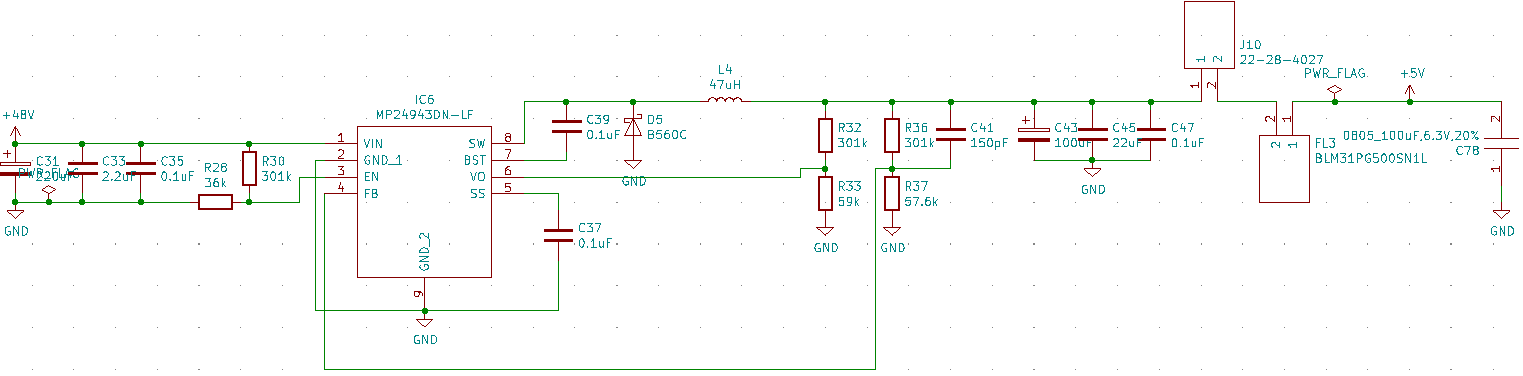
\includegraphics[width=\textwidth]{graphics/Schema_Speisung_5V.png}
	\caption{Schema der 5V Speisung}
	\label{fig:Schema_Speisung_5V}
\end{figure} 

\paragraph{Funktionsbeschrieb der Schaltung}\mbox{}\\

Auch bei der 5V Speisung wurde mittels R29 \& R31 ein Spannungsteiler realisiert, welcher das IC gemäss Kapitel \ref{subsubsec:12V Speisung} auf aktiv setzt.

Das Widerstandsverhältnis von R41 \& R42, welches die Ausgangsspannung definiert, wurde gemäss Formel \ref{equ:Ausgangsspannung_12V} berechnet. Somit ergeben sich für R41=301k$\Omega$ und für R42=57.6k$\Omega$, Was einer Ausgangsspannung von 4.98V entspricht. 

Beim Überspannungsschutz musste darauf geachtet werden, dass der Mikrokontroller AtMega2560-16AU nur in einem Spannungsbereich von 4.5V-5.5V betrieben werden darf. Die maximal verträgliche Eingangsspannung liegt laut Datenblatt bei 6V. Somit muss der Überspannungsschutz so gestaltet werden, dass die Schwelle von 6V nicht überschritten werden kann. Um dies erreichen zu können, wurde für R36=301k$\Omega$ und R37=53k$\Omega$ gewählt. Gemäss Formel \ref{equ:Vovp_12V} erhält man so eine Überspannungsschutzschwelle von 6V. 

Der interne Oszillator läuft wiederum bei einer Frequenz von 100kHz. Bei der ausgewählten Spule L4 von 47$\mu$H erhält man mittels Formel \ref{equ:12V_Spulenberechnung} ein $\Delta$I$_{L}$ von 0.953A. Auch hier gilt gemäss Datenblatt, dass die gewählte Spule auf mindestens 125\% des maximalen Ausgangsstroms von 3A ausgelegt werden soll. Auch der Gleichstromwiederstand der Spule sollte $ \leq \ $ 200m$\Omega$  sein. 

Mit den Kondensatoren C46, C48 \& C50 wird die Ausgangsspannung zum Abschluss auch noch geglättet. Bei den Eingangskondensatoren, sowie den Ausgangskondensatoren sollte es sich um low ESR Typen handeln. Auch hier wurde noch zum Abschluss ein Ferrit implementiert, welcher allfällige hochfrequente Störungen herausfiltern soll.

Auch bei der 5V Speisung wurde ein Jumper zu Testzwecken und zwei LED's implementiert. Ausserdem findet sich auch hier wieder ein Ferrit FL3, welcher letzte Störungen beseitigen soll. 




\subsubsection{3.3V Speisung}
\label{subsubsec:3.3V Speisung}

Um die Treiber der Motorenansteuerung, das Wireless-/Bluetoothmodul, die SD-Karte und die RFID-Schaltung zu betreiben, wird zusätzlich eine 3,3V-Speisung verbaut. Da es sich dabei nicht um  Leistungstreibende Elemente handelt, genügt ein einfacher Linearregler, der von der 5V-Speisung aus betrieben wird. 

\paragraph{Schema}\mbox{}

Bei dem Linearregler handelt es sich konkret um den LF33CDT-TRY von STMicroelectronics. Dieser hat eine fixe Ausgangsspannung von 3.3V bei einem maximalen Strom von 1A. Das dazugehörige Schema kann in Abbildung \ref{fig:Schema_Speisung_3.3V} begutachtet werden.

\begin{figure}[h!]
	\centering
	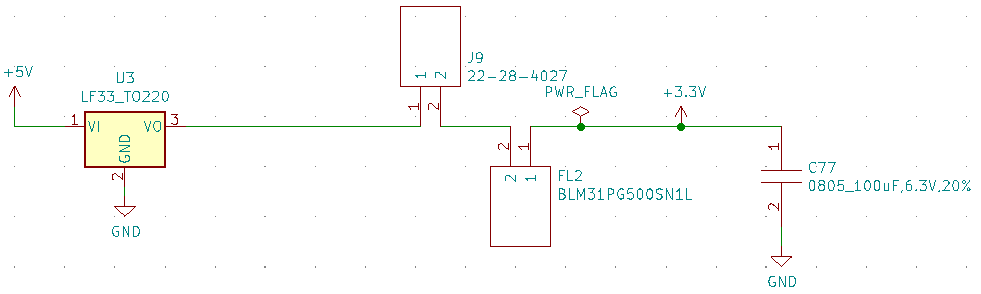
\includegraphics[width=0.5\textwidth]{graphics/Schema_Speisung_3,3V.png}
	\caption{Schema der 3.3V-Speisung}
	\label{fig:Schema_Speisung_3.3V}
\end{figure} 


\paragraph{Funktionsbeschrieb der Schaltung}\mbox{}

Der Linearregler benötigt keine spezielle Beschaltung. Er wird lediglich an die 5V Speisung angeschlossen. Am Eingang und am Ausgang ist ein Entstörkondensator implementiert. 

Wie bei der 12V-Speisung in Kapitel \ref{subsubsec:12V Speisung} und der 5V-Speisung in \ref{subsubsec:5V Speisung} wurde ein Jumper, sowie zwei LED's implementiert. Ein Ferrit FL1 filtert letzte Störungen heraus.

\clearpage
\subsection{Motor}
\label{subsec:Motor}

Um ein Glas während der Zubereitung hin- und her zu bewegen, wird eine Antriebsgruppe benötigt. Die Auswahl der Motorengruppe wurde mit dem Dozenten ausgewählt. Der Entscheid fiel dabei auf den Brushless DC-Motor AKM22h von Sigmatec. Auch dessen Ansteuerung ergab sich durch die schon vorhandenen EVAL-Boards mit dem FOC-Treiber (TMC4671) und der universal H-Brücke (UPS 10A70V). Im Projekt 6 wird anstelle der universellen H-Brücke ein Gate-Treiber (TMC6200) verwendet, welcher gemäss Kapitel \ref{subsubsec:Gate-Treiber} diverse Vorzüge hat. Das benötigte Feedback über die Lage des Rotors wird vom ABN-Encoder (AMT332S-V) geliefert. Zwei Shunts geben Auskunft über die Bestromung der Spulen. Auf die erwähnten Komponenten wird im Folgenden eingegangen. Abbildung \ref{fig:Blockdiagramm_TMC4671_und_TMC6200} zeigt, wie die Komponenten zusammenhängen.

\begin{figure}[H]
	\centering
	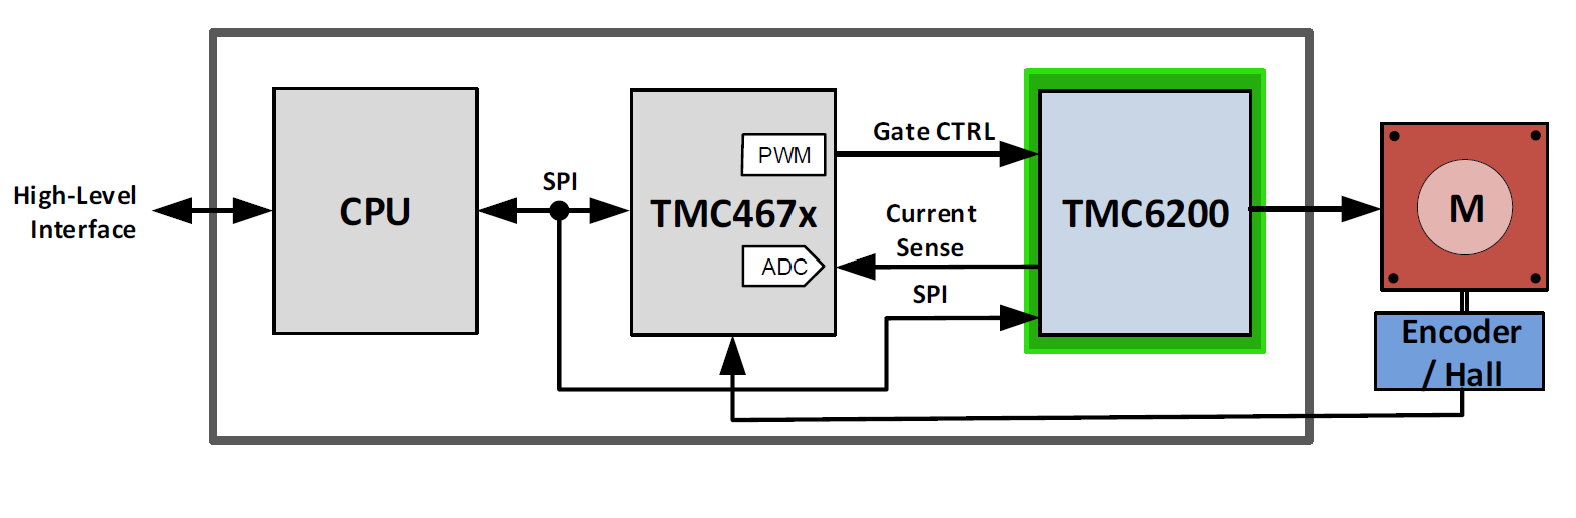
\includegraphics[width=0.8\textwidth]{graphics/Blockdiagramm_TMC4671_und_TMC6200}
	\caption{Blockschaltbild Konfiguration IC's mit BLDC und Encoder. \cite[S.1]{trinamicmotion_control_gmbh__co_kg_tmc6200_2019}}
	\label{fig:Blockdiagramm_TMC4671_und_TMC6200}
\end{figure}

%Es wurde darauf geachtet, dass der Aufbau des Prints dem Testaufbau entspricht. In Abbildung \ref{fig:Blockdiagramm_Motorengruppe} wird ein detaillierteres Blockschaltbild gezeigt, welches den Aufbau eher nach Funktionen beschreibt.

%\begin{figure}[H]
%	\centering
%	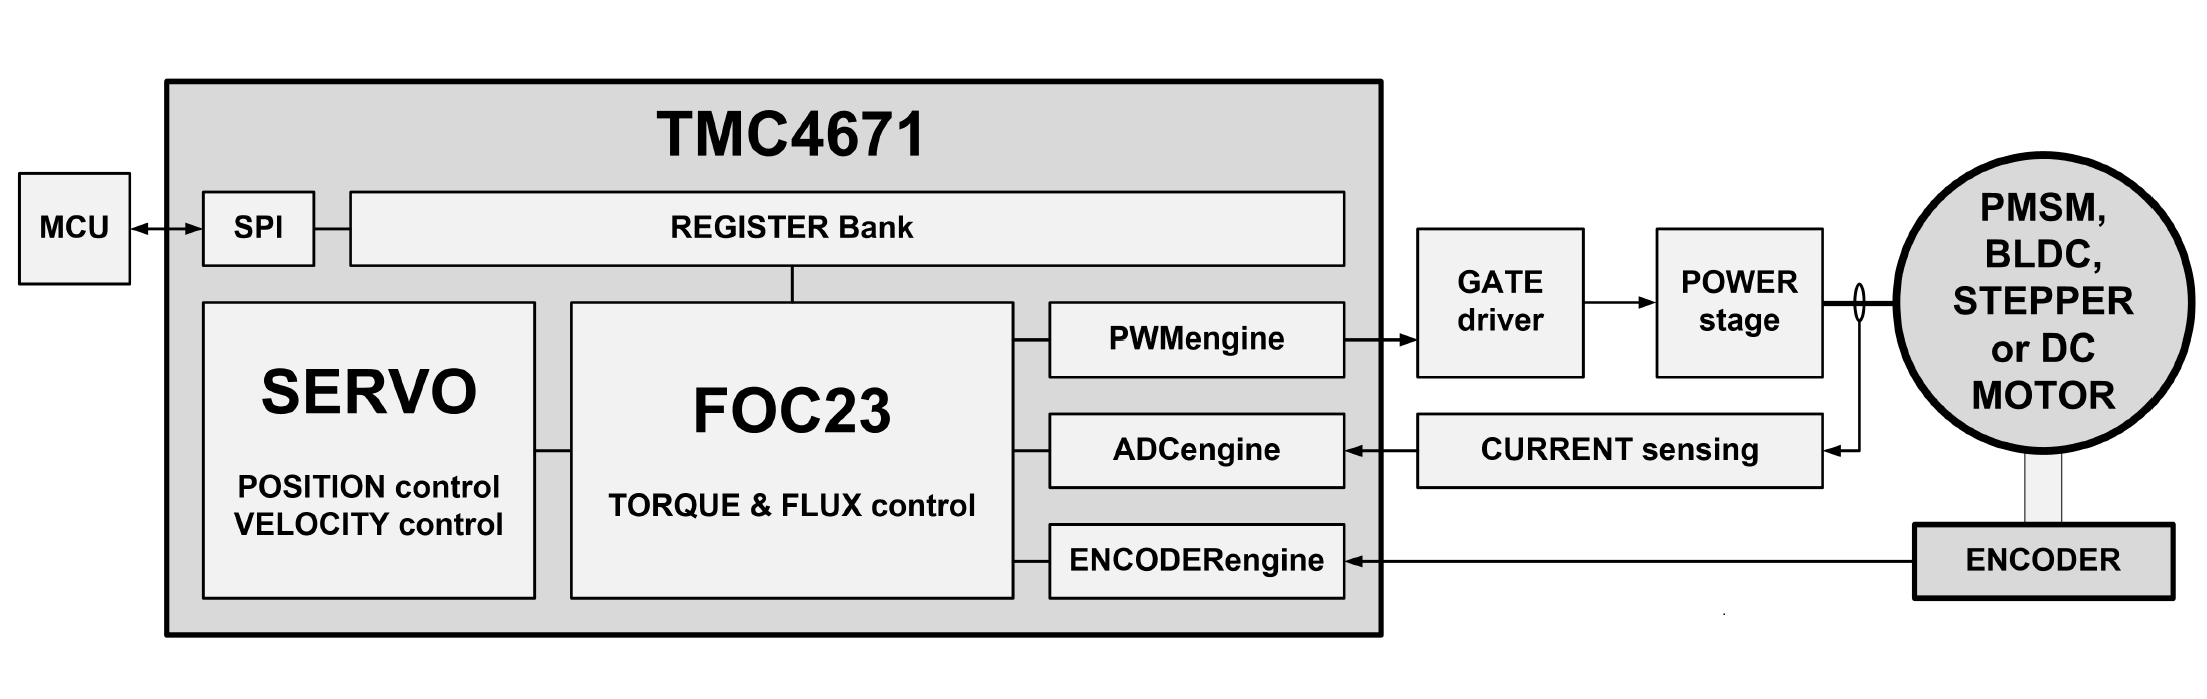
\includegraphics[width=0.8\textwidth]{graphics/Blockdiagramm_Motorengruppe}
%	\caption{Blockschaltbild Motorengruppe nach Funktionen. \cite[S.1]{trinamicmotion_control_gmbh__co_kg_tmc4671_2019}}
%	\label{fig:Blockdiagramm_Motorengruppe}
%\end{figure}

%\begin{table}[H]
%\center
%\begin{tabular}{|lll|l|}
%\hline
%\textbf{Kennzeichnung} & & \textbf{Bauteil} & \textbf{Funktion} \\
%\hline
%TMC4671 & = & Trinamic TMC4671 & FOC-Treiber \\
%GATE driver & = & Trinamic TMC6200 & Gate-Treiber \\
%POWER stage & = & Trnamic UPS 10A70V & H-Brücke \\
%Current sensing & = & UPS 10A70V ==> TMC6200 & Messung Phasenströme \\
%PMSM/BLDC & = & Sigmatec AKM22h & BLDC \\
%ENCODER & = & CUI devices ATS33 & ABN-Encoder \\
%\hline
%\end{tabular}
%\end{table}
%\newpage

\subsection{BLDC und H-Brücke}
\label{subsec:BLDC und H-Brücke}



\subsubsection{ABN-Encoder}
\label{subsubsec:ABN-Encoder}



\clearpage
\section{Einleitung}
\label{sec:Einleitung}



\clearpage
\section{Einleitung}
\label{sec:Einleitung}



\subsubsection{Pumpen}
\label{subsubsec:Pumpen}



\input{sections/5_3_1_Durchflussmessgeräte}

\clearpage
\subsection{Benutzerschnittstellen}
\label{subsec:Benutzerschnittstellen}



\subsubsection{Display}
\label{subsubsec:Display}

Der Benutzer bedient den PartyMixer via dem Nextion Touch-Display. Dabei handelt es sich um das Display NX8048T070. Das GUI basiert dabei auf den Funktionen, die in der Software Nextion Editor zur Verfügung gestellt werden. Die Funktionen umfassen:
\begin{itemize}
\item Erstellen von Seiten, die auf dem Display angezeigt werden.
\item Setzen von Buttons, Slider und Textfeldern auf den Seiten.
\item Speichern von Grafiken, die auf den Seiten angezeigt werden.
\item Kommunizieren über UART um Aktionen auszulösen.
\end{itemize}

\paragraph{Schema}\mbox{}

Um das Display mit der Leiterplatine zu verbinden, braucht es einen Stecker und einen Stützkondensator nahe der Pins am Spannungsausgang, um die Versorgungsspannung zu glätten. Auf eine Abbildung wird verzichtet, der Stecker für das Display ist jedoch im Schema auf Seite 7 zu sehen, welches im Anhang Kapitel \ref{Appendix:Schema_Print} eingefügt ist.

\paragraph{Funktionsbeschrieb der Schaltung}\mbox{}

Die Funktionen werden durch das Stützen der Versorgungsspannung mit dem Kondensator und der Anbindung des Displays an die Leiterplatine gegeben.

\newpage
\subsubsection{ESP}
\label{subsubsec:ESP}

Für die Implementierung des WiFi's wird das ESP32 verwendet. Die Hauptfunktion im Schema ist die Kommunikation mit dem Mikrocontroller über die zweite serielle Schnittstelle. Die Ansteuerung zum Schreiben des Programmspeichers muss so gestaltet werden, dass der Boot-Modus automatisch gestartet werden kann, wenn ein Code hochgeladen werden soll. Dies hat eine zusätzliche Schaltung zur Folge. 

\paragraph{Schema (WiFi-Modul)}\mbox{}

In Abbildung \ref{fig:Schema_ESP32} wird das Schema rund um das ESP32 an sich gezeigt. Es beinhaltet Stütz- und Filterkondensatoren sowie einige Pull-up- und Pull-down-Widerstände, welche verwendet werden, um einen vordefinierten Grundzustand beim Booten des ESP32-Moduls zu erreichen (Strapping-Pins). Weiter gibt es einen Kondensator, welcher dazu da ist, bei gewünschter Zeit in den Boot-Modus zu gelangen. 

\begin{figure}[h!]
	\centering
	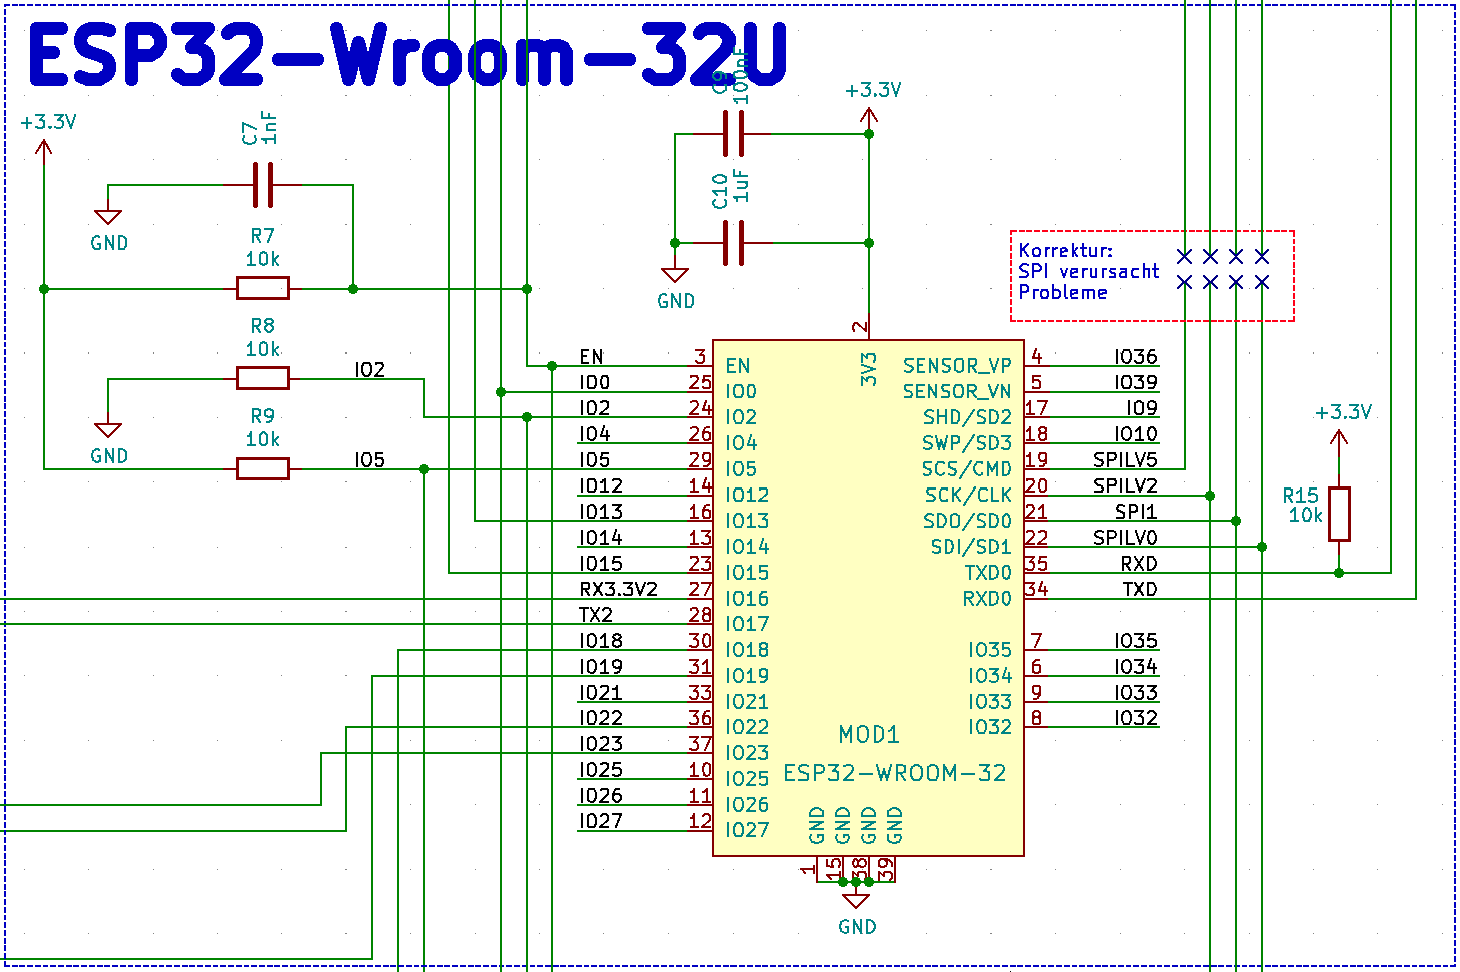
\includegraphics[width=\textwidth]{graphics/Schema_ESP32}
	\caption{Schema ESP32-Wroom-32U.}
	\label{fig:Schema_ESP32}
\end{figure}

\paragraph{Funktionsbeschrieb der Schaltung (WiFi-Modul)}\mbox{}

Das ESP32 ist mit MOD1 beschriftet, es übernimmt die in Kapitel \ref{subsec:Wirelessmodul} beschriebenen Funktionen. Die Kondensatoren C9 und C10 dienen zu Stütz- und Filterzwecken am Spannungseingang.  Über den EN-Pin wird das Modul ein- und ausgeschaltet (acitve high). Der Widerstand R7 ist ein Pull-Up für Chip-Enable. Die Widerstände R8, R9, R10 und R11 sind an die Strapping-Pins angeschlossen. Über diese werden beim Aufstarten des ESP32 der Boot-Modus, die Versorgungsspannung von VDD\_SDIO\footnote{Secure Digital Input Output}-Slave (Erweiterung der SD-Spezifikationen) und andere Initialisierungseinstellungen konfiguriert. Details zu den Konfigurationen sind in Tabelle \ref{tab:Strapping_pins} aufgelistet\footnote{https://www.espressif.com/sites/default/files/documentation/esp32\_datasheet\_en.pdf S.13}. Der Widerstand R15 zieht U0TXD auf HIGH. Aus Tabelle \ref{tab:Einfluss_Pins_auf_Boot_Modus} ist ersichtlich, dass dieser für den normalen Boot-Modus auf HIGH sein muss. Für den Download-Boot-Modus hat dieser kein Einfluss. Mit dem Kondensator C7 wird sichergestellt, dass nach einem Reset der Bootmodus gestartet werden kann. Wird der Reset-Pin au LOW gezogen, so entlädt sich der Kondensator. Sobald der Reset-Pin auf HIGH gezogen wird, dauert es länger, bis ein logic High-Zustand am CMOS-Eingang erkannt wird. Wird der Pin IO0 auf LOW gezogen, bevor der Enable-Pin nach einem Reset einen HIGH-Zustand erreicht, so wird das ESP32 in den Download-Boot-Modus gesetzt. Um automatisch in diesen Boot-Modus zu kommen benötigt es eine Logik, welche im Folgenden erklärt wird.

\paragraph{Schema (Automatische Boot-Logik)}\mbox{}

In Abbildung \ref{fig:Schema_ESP32_Flashbuttons} wird die Schaltung gezeigt, welche verwendet wird, das ESP32-Modul in den gewünschten Boot-Zustand zu bringen. Für die Beschaltung der automatischen Boot-Logik benötigt es eine Schaltung mit DTR und RTS als Inputs vom USB-UART-Converter her und EN und IO0 als Outputs auf das ESP32. Die Buttons können bei Bedarf verwendet werden, sind für den automatischen Boot-Modus jedoch nicht zwingend nötig. Sie könnten dazu verwendet werden, manuell in den Bootmodus zu gelangen.\\
Die Widerstände R20 und R21 sind Vorwiderstände an der Basis der Transistoren Q1 und Q2. R22 und R23 sind Pull-Up-Widerstände für die EN- und IO0-Leitung. Die Kondensatoren C13 und C12 dienen zum entprellen. Die Widerstände R25 und R24 begrenzen den Strom bei Drücken der Buttons S1 und S2.

\begin{figure}[h!]
	\centering
	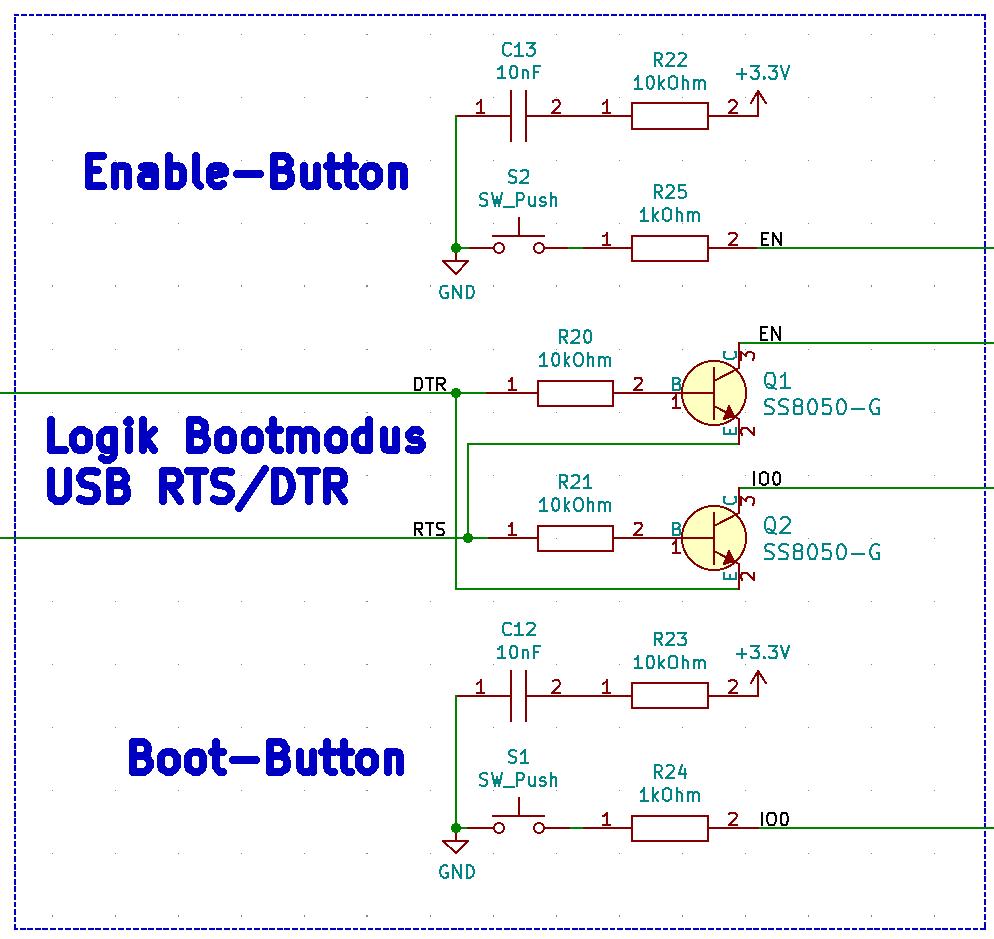
\includegraphics[width=0.7\textwidth]{graphics/Schema_ESP32_Flashbuttons}
	\caption{Schema ESP32-Wroom-32U.}
	\label{fig:Schema_ESP32_Flashbuttons}
\end{figure}

\newpage

\paragraph{Funtionsbeschrieb der Schaltung (Automatische Bootlogik)}\mbox{}



\subsubsection{USB-C}
\label{subsubsec:USB-C}



\subsubsection{RFID}
\label{subsubsec:RFID}


\subsection{Beleuchtung}
\label{subsec:Beleuchtung}



\subsection{Mikrocontroller}
\label{subsec:Mikrocontroller}

Der Mikrocontroller ist die Seele, das Gehirn der Maschine. Er muss in der Lage sein mit allen Komponenten auf der Platine zu kommunizieren, die Tasks zu verarbeiten und abhandeln. Der ATMega2560 übernimmt diese Aufgabe.

\paragraph{Schema}\mbox{}

Das Schema besteht aus dem Mikrocontroller IC8 mit den fünf Stützkondensatoren C62, bis C66 an den Spannungseingängen. Mit dem Full Swing Oscillator Crystal Y2 und den Kondensatoren C58 und C59 wird eine Frequenz von 16MHz generiert. Der Reset-Button SW3 dient dazu, den Mikrocontroller manuell neu zu starten. Der dazugehörige Kondensator C81 entprellt den Button und der Widerstand R74 zieht die Leitung mittels Pull-up auf VCC. Mittels dem ISP-Stecker kann über einen Programmer, z.B AVR MKII, auf den Mikrocontroller zugregriffen werden. Der DIP-Switch ist dazu da, die SPI-Leitungen von der ISP-Schnittstelle zu trennen. Die LED D9 gibt Auskunft ob Spannung am Mikrocontroller anliegt.

\begin{figure}[!h]
\center
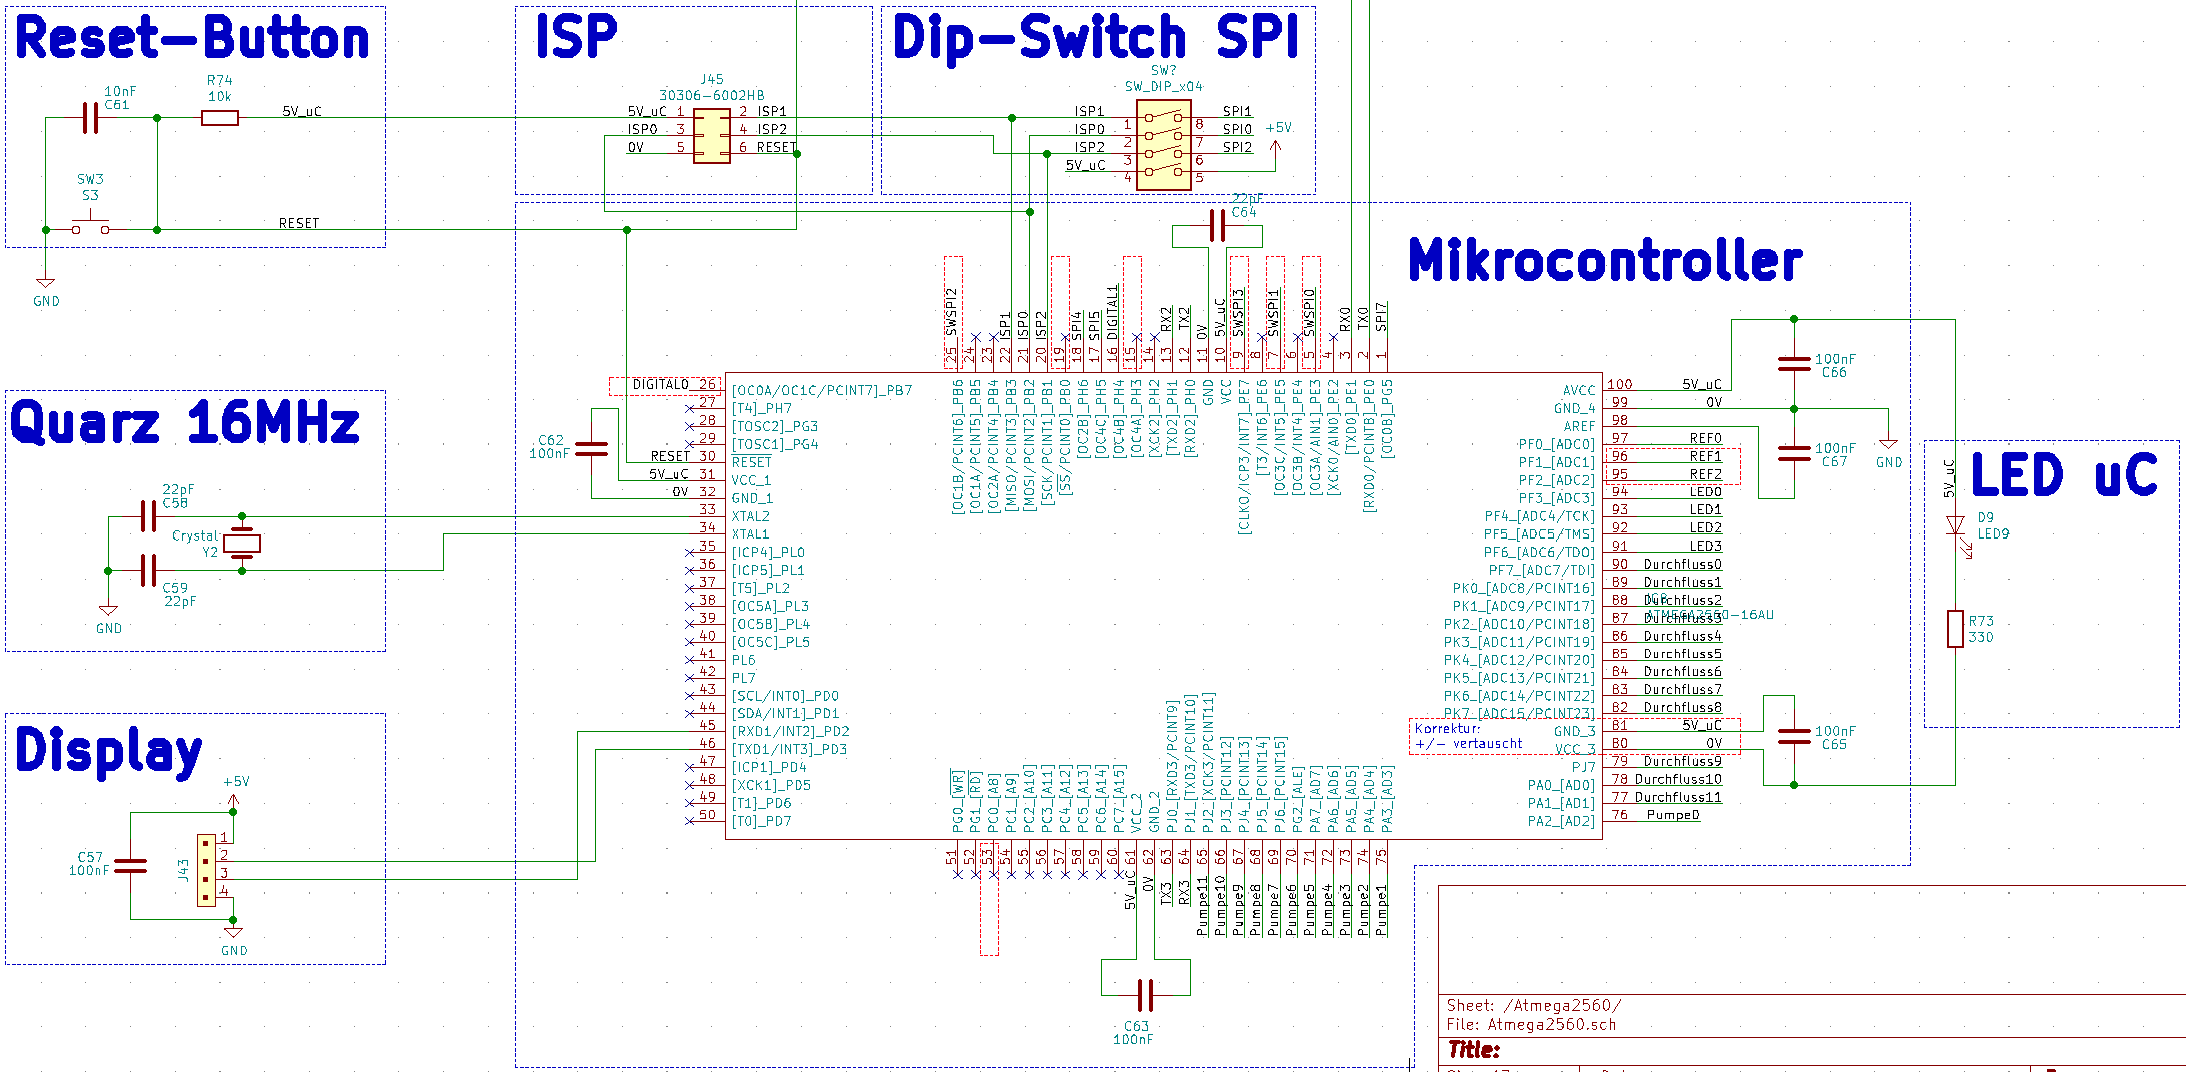
\includegraphics[width = \textwidth]{graphics/Schema_uC}
\caption{Schema Mikrocontroller}
\label{fig:Schema_uC}
\end{figure}

\paragraph{Funktionsbeschrieb der Schaltung}\mbox{}

Die Stüzkondensatoren halten die Spannung am Mikrocontroller konstant. Die Quarz-Schaltung wird gebraucht, da der Mikrocontroller nur eine 8MHz-RC-Clock integriert hat, jedoch mit 16MHz gearbeitet wird. Der Reset-Button zieht in gedrücktem Zustand die Reset-Leitung auf GND. Dabei entlädt sich der Kondensator schnell, da er kurzgeschlossen wird. In offenem Zustand lädt sich der Kondensator über den Widerstand R74 mit einer Zeitkonstante von $\tau = R_{74} \cdot C_{81} = 100us$. Die Trennung von SPI und ISP wird gemacht, sodass gewährleistet ist, dass bei der Inbetriebnahme des Mikrocontrollers die restlichen SPI-kommunikationsfähigen Komponenten nicht mitreden können. Zudem kann die 5V-Versorgungsspannung des Mikrocontroller vom Rest der Platine getrennt werden, sodass dieser auch bei ausgeschalteter Board versorgt werden kann, ohne die anderen Komponenten zu speisen. Deswegen auch die Betriebs-LED.

\section{Inbetriebnahme}
\label{sec:Inbetriebnahme}

Ein essentieller Teil der Entwicklung ist die Inbetriebnahme. Dabei wurden die Teilsysteme nacheinander in Betrieb genommen. Die einzelnen Systeme wurden dann in ihren wichtigsten Funktionen geprüft und für den Einsatz vorbereitet. In den folgenden Kapiteln wurden die einzelnen Teilsysteme der Cocktailmaschine in Betrieb genommen. 

\subsection{Speisungen}
\label{subsec:Inbetriebnahme_Speisungen}

Um die Speisungen in Betrieb nehmen zu können, ist gemäss Kapitel \ref{subsec:Speisungen} ein Jumper in die Schaltung implementiert worden, welcher die Speisungen von der übrigen Hardware trennt. Ausserdem sind Status-LED's verbaut, welche den korrekten Betrieb anzeigen sollen. Da es sich bei der 48V-Speisung um ein fertiges Netzteil handelt, musste dieses nicht grossartig in Betrieb genommen werden. Die einzige Einstellung, welche vorgenommen werden musste, ist die Feinjustierung der Ausgangsspannung mittels Drehregler am Netzteil.


\subsubsection{12V Speisung}
\label{subsubsec:Inbetriebnahme_12V_Speisungen}

Die 12V Speisung wurde für die Inbetriebnahme vom übrigen System abgekoppelt. Da diese aus der 48V-Speisung generiert wird, wurde lediglich diese vorgeschaltet. Beim Einschalten des Netzteils war der korrekte Betrieb am Status-LED sichtbar. Eine Messung mit dem Voltmeter bestätigte dies. Um allfällige Rippel sehen zu können, wurde noch mit dem Oszilloskop gemessen.



\subsubsection{5V Speisung}
\label{subsubsec:Inbetriebnahme_5V_Speisungen}

Simultan zur 12V-Speisung wurde die 5V-Speisung in Betrieb genommen. Auch bei dieser Speisung wurde lediglich das Netzteil vorgeschaltet und das restliche System abgeschnitten. Auch hierbei leuchtete das Status-LED sofort auf. Um zu verifizieren ob die richtige Spannung anliegt, wurde dies auch hier mit einem Voltmeter geprüft.

\subsubsection{3.3V Speisung}
\label{subsubsec:Inbetriebnahme_3.3V_Speisungen}



\subsection{Motor}
\label{subsec:Inbetriebnahme_Motor}



\input{sections/6_2_0_BLDC_&_H-Brücke}

\clearpage
\section{Einleitung}
\label{sec:Einleitung}



\subsubsection{Treiber}
\label{subsubsec:Inbetriebnahme_Treiber}





\subsection{Flüssigkeitsbeförderung}
\label{subsec:Inbetriebnahme_Flüssigkeitsbeförderung}



\subsubsection{Pumpen}
\label{subsubsec:Inbetriebnahme_Pumpen}



\input{sections/6_3_1_Durchflussmessgeräte}

\clearpage
\section{Einleitung}
\label{sec:Einleitung}



\clearpage
\section{Einleitung}
\label{sec:Einleitung}



\subsubsection{ESP}
\label{subsubsec:Inbetriebnahme_ESP}



\clearpage
\section{Einleitung}
\label{sec:Einleitung}



\subsubsection{RFID}
\label{subsubsec:Inbetriebnahme_RFID}


\subsection{Beleuchtung}
\label{subsec:Inbetriebnahme_Beleuchtung}

Die Farbe und Helligkeit der Beleuchtung wird mit einem PWM-Signal geregelt. Das PWM-Signal wird erzeugt mittels Timer Interrupts, damit Regelung parallel neben dem Programfluss geschehen kann. Insgesamt benötigt es fünf Timer, um das LED-Band anzusteuern. Jeweils einen für jede Farbe und einen um durch den Rainbow-Modus zu interieren.

\subsubsection{PWM-Signale LED}

Das PWM-Signal für die LEDs wird mit einer Frequenz von 10 kHz initialisiert. Um dies zu erreichen, wird Formel \ref{equ:Timer_Max_1} umgestellt nach \ref{equ:Timer_Max_2}. Der Prescaler ist N = 1. Das Ergebnis wird im Register OCRnA gespeichert, wodurch der Timer $1/10kHz = 100\mu s$ benötigt, bis ein Timer\_nx Compare-Interrupt ausgelöst wird.

\begin{equation}
f_{OC_{max}} = \frac{f_{clk_{I/O}}}{2 \cdot N \cdot (1+OCR_{nA})}
\label{equ:Timer_Max_1}
\end{equation}

umgestellt nach OCR\_nx:

\begin{equation}
OCR_{nx} = \frac{f_{clk_{I/O}}}{2 \cdot N \cdot f_{OC_{max}}} - 1 = \frac{16MHz}{2 \cdot 1 \cdot 10kHz} - 1 = 799
\label{equ:Timer_Max_2}
\end{equation}

Damit das Hochzählen des Counters nach erreichen von OCRnA wieder bei null beginnt, wird der Timer im CTC-Mode betrieben. Das Register OCRnA stellt so den maximalen Wert des Counters dar. Dies ist in Abbildung \ref {fig:Timer_CTC_Mode} und \ref{fig:Timer_CTC_Timing_Diagram} zu sehen.

\begin{figure}[h!]
	\centering
	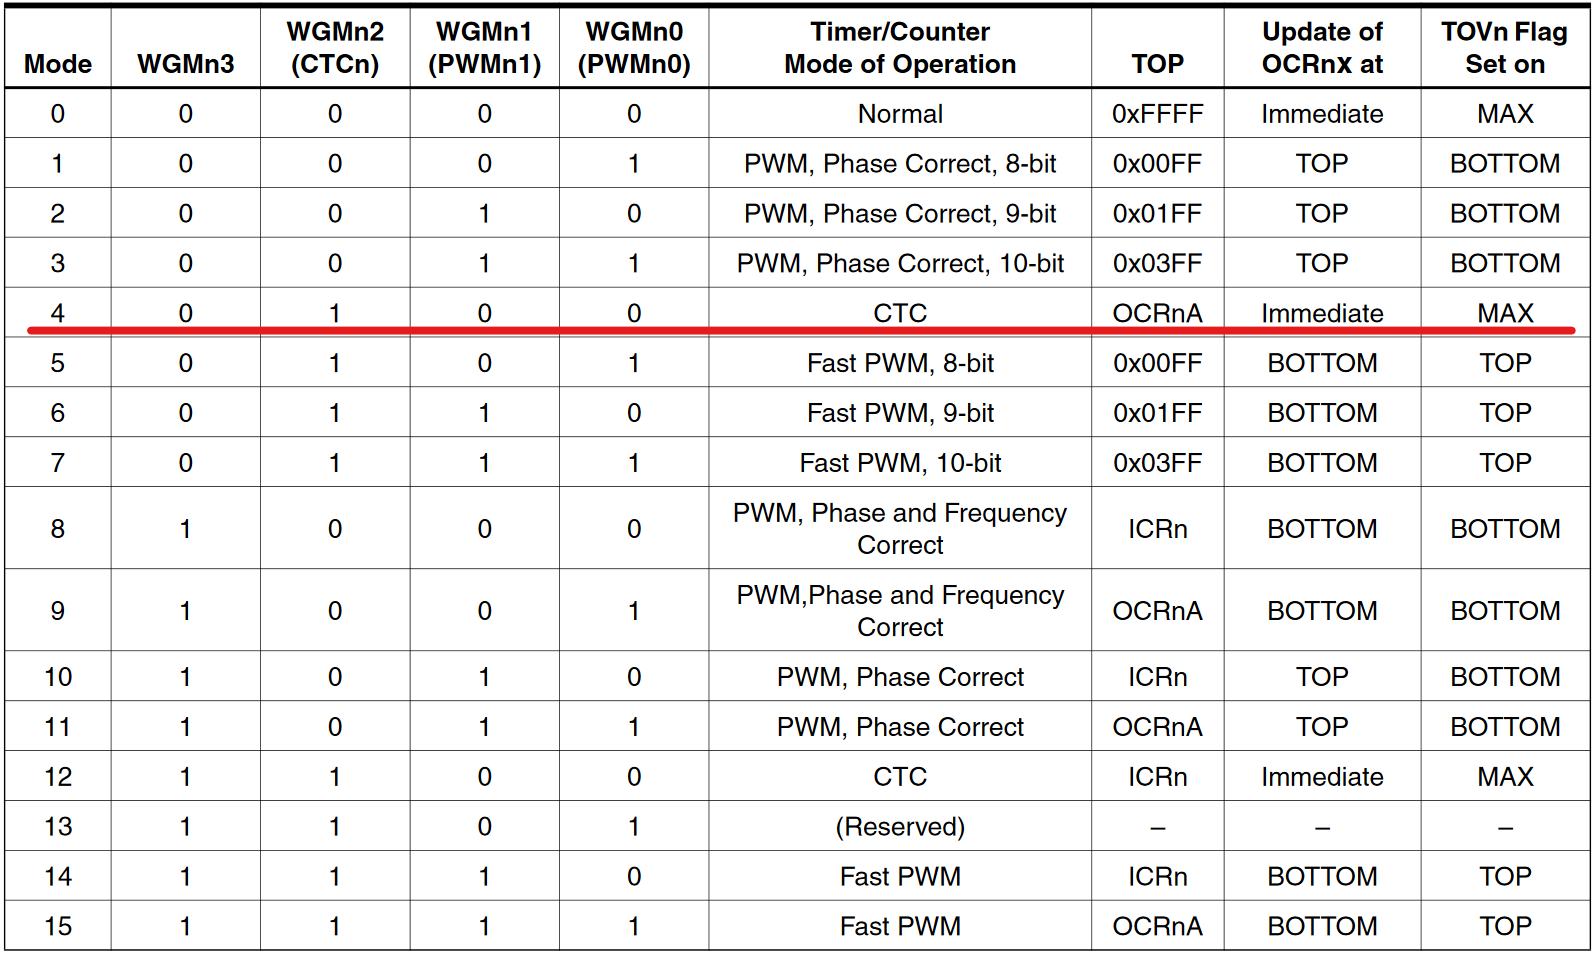
\includegraphics[width=\textwidth]{graphics/Timer_CTC_Mode}
	\caption{Timing-Diagramm CTC-Mode. OCnx nicht angeschlossen, Pin wird softwaremässig getoggelt.}
	\label{fig:Timer_CTC_Mode}
\end{figure}

\begin{figure}[h!]
	\centering
	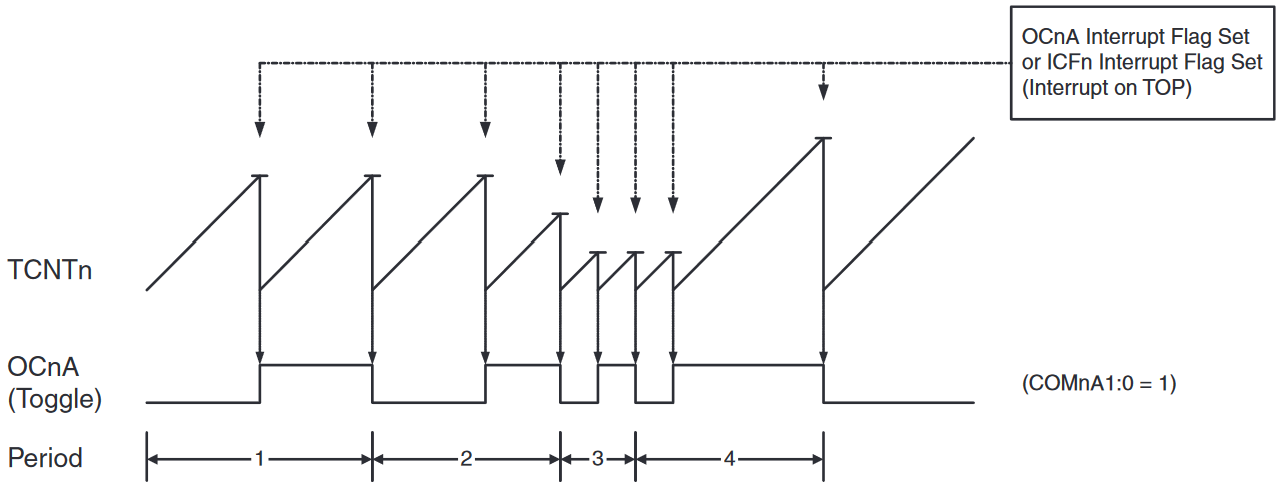
\includegraphics[width=\textwidth]{graphics/Timer_CTC_Timing_Diagram}
	\caption{Timing-Diagramm CTC-Mode. OCnx nicht angeschlossen, Pin wird softwaremässig getoggelt.}
	\label{fig:Timer_CTC_Timing_Diagram}
\end{figure}

\todo{cites: Atmel Datenblatt S.146}

Der Duty-Cycle wird Prozentual zum OCRnA-Register gesetzt. Wird für den berechneten Wert ein Duty-Cycle von 50\% vorgegeben, ergibt sich für das OCRnB-Register den Wert $(800 / 2) -1 \approx 399$. So wird nach der Hälfte der Hochzählzeit ein zweiter Compare-Interrupt ausgelöst, welcher jedoch kein Einfluss auf das Counter-Register hat.

Nun muss in beiden der erwähnten Interrupt-Routinen das gewünschte LED getoggelt werden. In der ersten Interruptroutine mit dem OCRnA-Compare-Register wird die LED eingeschaltet, in der zweiten Interruptroutine mit dem OCRnB-Compare-Register wird die LED ausgeschaltet.

Möchte man nun die Helligkeit angepasst werden, kann ein Wert zwischen 0 und OCRnA ausgewählt werden und damit das Register OCRnB beschrieben werden.

\todo{cite:  Formel - Atmega datenblatt S.121 }
\todo{cite:  Prescaler - Atmega datenblatt S.129 }
\todo{cite:  CTC-Mode - Atmega datenblatt S.145 }
\todo{cite:  CTC-Timing-Diagramm - Atmega datenblatt S.146 }

Der Wert für das OCRnA-Register ist folglich 799. Ein OCRnB-Register wird nicht benötigt, da die Iteration nur ausgeführt wird, sobald ein OCRnA-Compara-Match-Interrupt ausgelöst wird.

\subsubsection{Custom-Funktion}

Bei der Custom-Funktion können die Farbwerte manuell definiert werden. So wird für eine bestimmte Farbe für jede LED-Farbe der entsprechende Wert in das OCRnB-Register geschrieben. Darf sich eine Farbe nicht verändern, so muss das OCRnB-Register den gleichen Wert behalten. Die Itearation durch den Rainbow-Algorithmus wird im Custom-Mode nicht benötigt.

\subsubsection{Rainbow-Funktion}

Die Farbe der RGB-LED soll nun jeweils fünf Sekunden brauchen, um einen Farbteil komplett ein- oder auszuschalten, was einen sanften Übergang im Farbkreis ermöglicht.

Im Rainbow-Loop gibt es sechs States. Zubeginn muss die grüne LED schon voll leuchten.
\begin{enumerate}
\item Start ==> Grün
\item Hochzählen des Rot-Anteils ==> Yellow
\item Runterzählen des Grün-Anteils ==> Rot
\item Hochzählen des Blau-Anteils ==> Magenta
\item Runterzählen des Rot-Anteils ==> Blau
\item Hochzählen des Grün-Anteils ==> Cyan
\item Runterzählen des Blau-Anteils ==> Grün
\item Repeat 2 - 7
\end{enumerate}

Es benötigt 800 Schritte um einen Farbteil komplett ein- und auszuschalten. Pro Interrupt wird ein Schritt hochgezählt. Mit Formel \ref{equ:Milli_S} kann direkt berechnet werden, mit welchem Wert das Compare-Register beschrieben werden muss, sodass es fünf Sekunden geht, bis 800 Schritte hochgezählt wurden.

\begin{equation}
OCR_{nx} = \frac{f_{clk_{I/O}}}{2 \cdot N \cdot f_{OC_{max}}} - 1 = \frac{16MHz}{2 \cdot 1024 \cdot \frac{5s}{800 Schritte}} - 1 \approx 48
\label{equ:Milli_S}
\end{equation}

Die Iteration durch den Rainbow-Modus wird folglich mit einer Frequenz von 160Hz initialisiert. In der Routine wird demnach alle 6.25ms der Duty-Cytle einer Farbe hoch oder runtergezählt, und das Timer-Compare-Register des entsprechenden LED-Timers angepasst.

\subsubsection{Vorgehen}

\begin{enumerate}
\item Benötigte Applikation aus dem Software-Ordner auf dem USB-Stick in Atmel Studio öffnen.\\
\textcolor{magenta}{Software\textrightarrow Atmega\textrightarrow 3\underline{ }LED\underline{ }Control\textrightarrow 1\underline{ }LED\underline{ }Testsoftware\textrightarrow LED}\\

\item Software hochladen:\\
\textcolor{blue}{AtmelStudio\textrightarrow Tools\textrightarrow Cocktailmixer}\\

\end{enumerate}

\newpage
\section{Software}
\label{sec:Software}



\clearpage
\section{Einleitung}
\label{sec:Einleitung}



\clearpage
\section{Einleitung}
\label{sec:Einleitung}



\section{Evaluation}
\label{sec:Evaluation}



\clearpage
\section{Einleitung}
\label{sec:Einleitung}



\subsection{Zielerreichung}
\label{subsec:Zielerreichung}



\clearpage
\section{Einleitung}
\label{sec:Einleitung}



\section{Schlusswort}
\label{sec:Schlusswort}



\section{Ehrlichkeitserklärung}\label{sec:Ehrlichkeitserklärung}
Mit der Unterschrift bestätigt der Unterzeichnende Projektleiter, dass die vorliegende Projektdokumentation selbstständig im Team und ohne Verwendung anderer, als der angegebenen Hilfsmittel verfasst wurde, sämtliche verwendeten Quellen erwähnt und die gängigen Zitierregeln eingehalten wurden. Eine Überprüfung der Arbeit auf Plagiate mithilfe elektronischer Hilfsmittel darf vorgenommen werden.


\vspace{20mm}


\begin{center}
		\renewcommand{\arraystretch}{1}
	\begin{tabular}{lp{5em}l} 
  
		
		Unterschrift:   && Ort, Datum: \\
		&&\\
		\hspace{5cm}   && \hspace{5cm} \\\cline{1-1}\cline{3-3}
		&&\\
		&&\\
		

  
  \ \\
 \end{tabular}
 \end{center}





\pagebreak


\clearpage
%%---BIBLIOGRAPHY------------------------------------------------------------------------
{\sloppypar
\printbibliography[heading=bibintoc]
\label{sec:lit}
%\selectlanguage{ngerman}				%ngerman or english
%\printbibliography
}

%%---APPENDIX----------------------------------------------------------------------------
\begin{appendix} 

\section{TMC4671}\label{Appendix:TMC4671}

\subsection{Standard-Schaltkreis TMC4671}

\begin{figure}[h!]
	\centering
	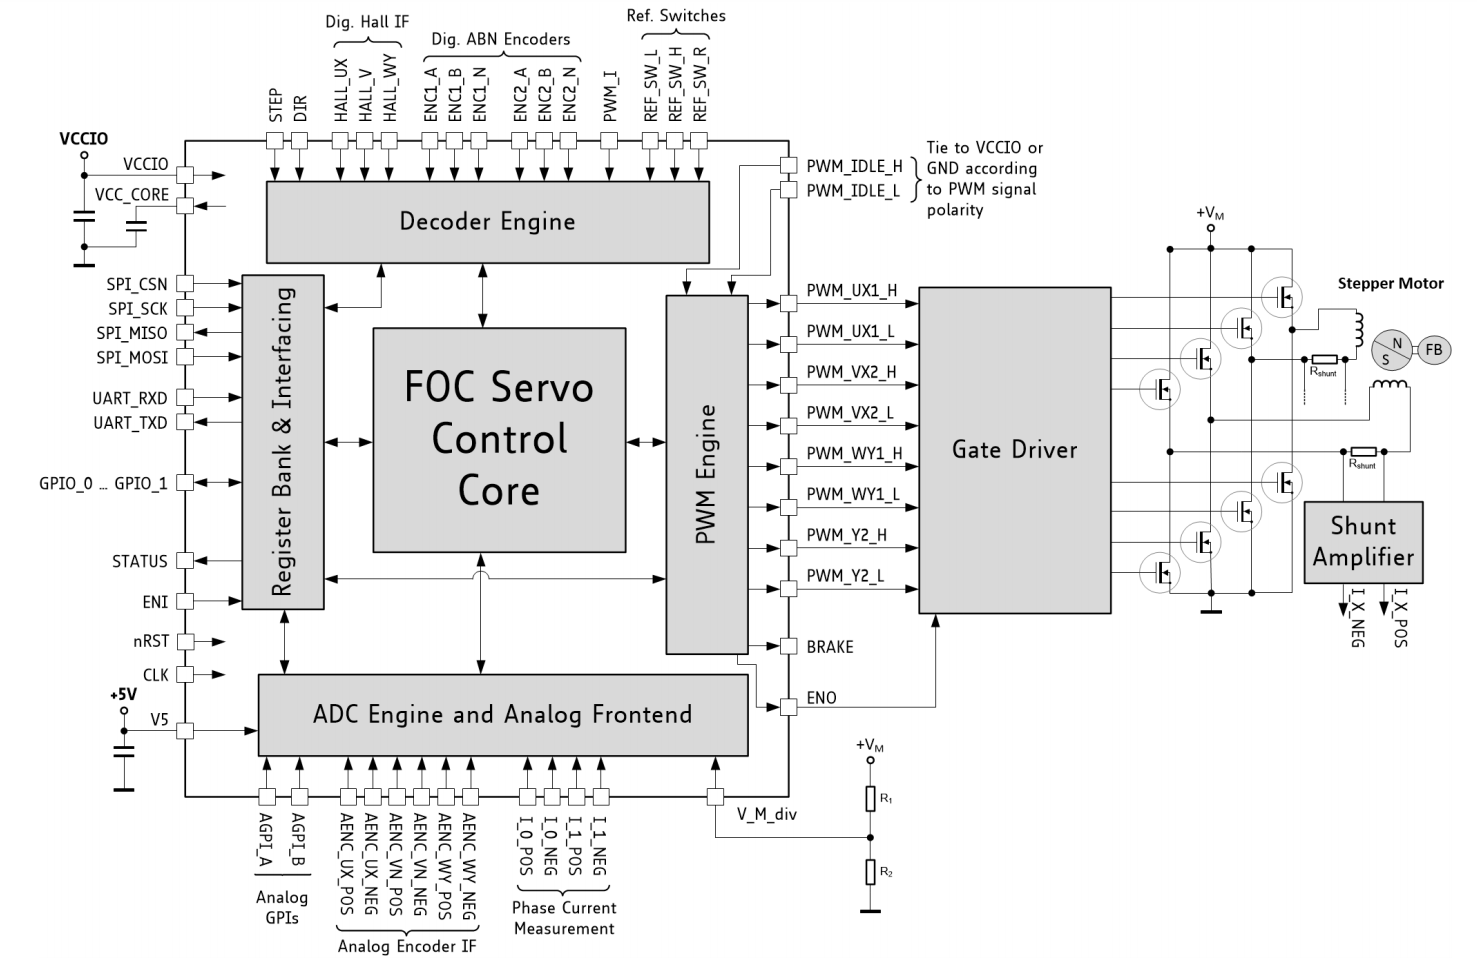
\includegraphics[width=0.8\textwidth]{graphics/Standard_Application_Cirquit_TMC4671}
	\caption{Standard-Anwendungs-Schaltung.}
	\label{fig:Schaltung_TMC4671}
\end{figure}
\todo{cite{TMC4671 Datenblatt}}

\subsection{Blockdiagramm TMC4671}

\begin{figure}[h!]
	\centering
	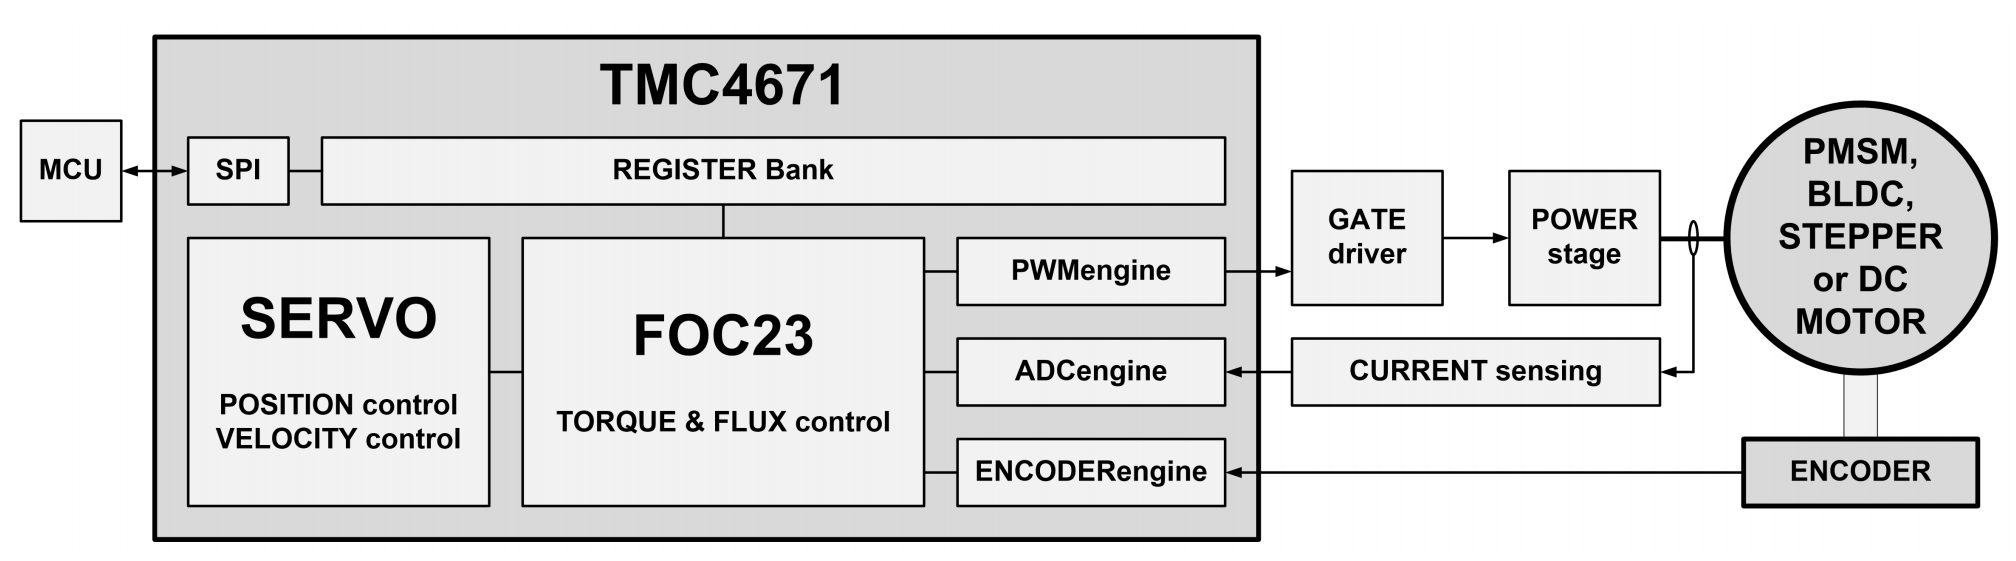
\includegraphics[width=0.8\textwidth]{graphics/Blockdiagramm_TMC4671}
	\caption{Blockdiagramm TMC4671.}
	\label{fig:Blockdiagramm_TMC4671}
\end{figure}

\todo{cite{TMC4671 Datenblatt}}

\newpage

\subsection{Inbetriebnahme Gate-Control}

\begin{figure}[h!]
\center
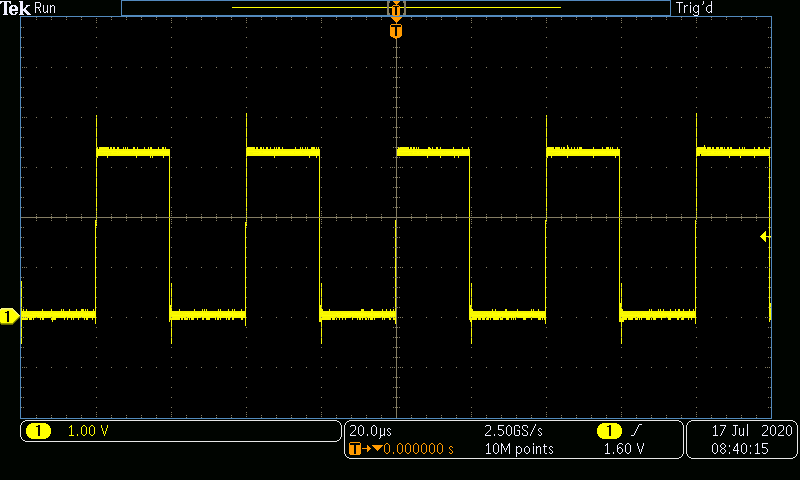
\includegraphics[width = 0.8\textwidth]{graphics/PWM_UX1_H}
\caption{Steuersignal PWM\_UX1\_H}
\label{fig:PWM_UX1_H}
\end{figure}

\begin{figure}[h!]
\center
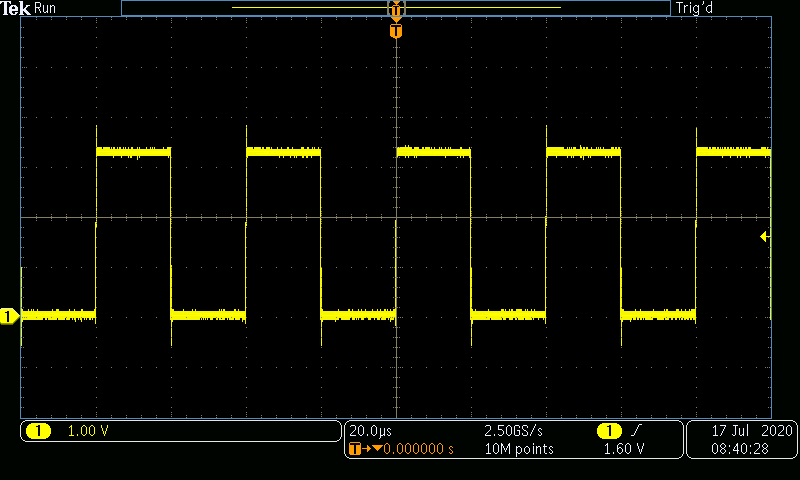
\includegraphics[width = 0.8\textwidth]{graphics/PWM_UX1_L}
\caption{Steuersignal PWM\_UX1\_L}
\label{fig:PWM_UX1_L}
\end{figure}

\newpage

\begin{figure}[h!]
\center
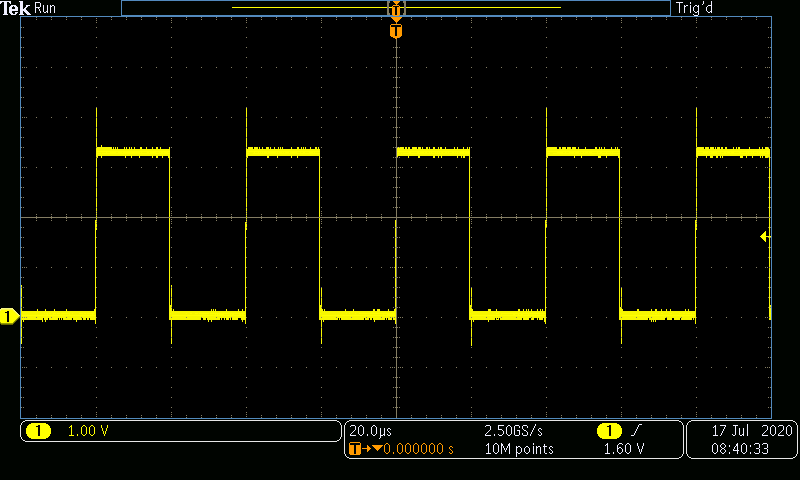
\includegraphics[width = 0.8\textwidth]{graphics/PWM_UX2_H}
\caption{Steuersignal PWM\_UX2\_H}
\label{fig:PWM_UX2_H}
\end{figure}

\begin{figure}[h!]
\center
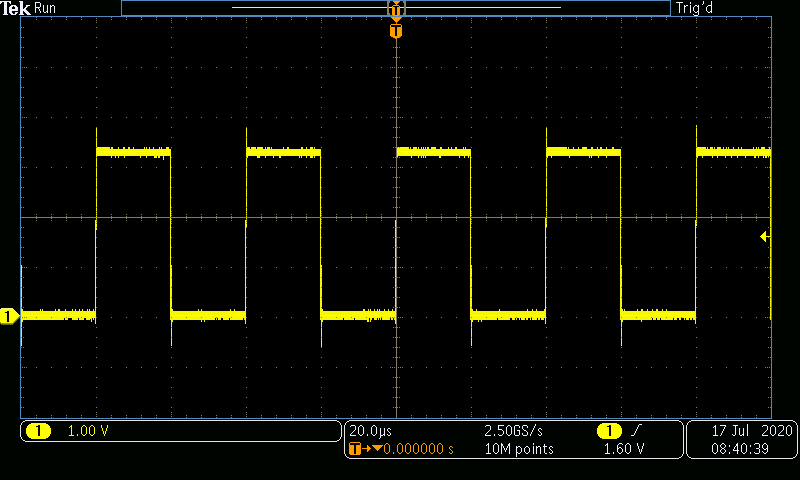
\includegraphics[width = 0.8\textwidth]{graphics/PWM_UX2_L}
\caption{Steuersignal PWM\_UX2\_L}
\label{fig:PWM_UX2_L}
\end{figure}

\newpage

\begin{figure}[h!]
\center
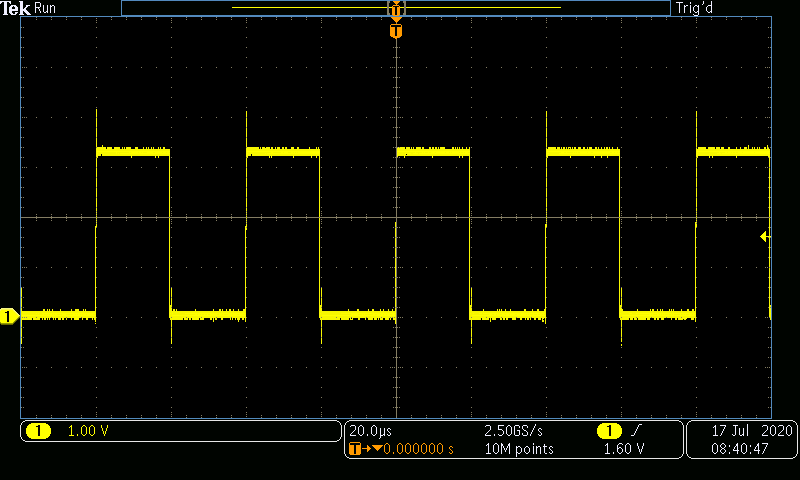
\includegraphics[width = 0.8\textwidth]{graphics/PWM_UX3_H}
\caption{Steuersignal PWM\_UX3\_H}
\label{fig:PWM_UX3_H}
\end{figure}

\begin{figure}[h!]
\center
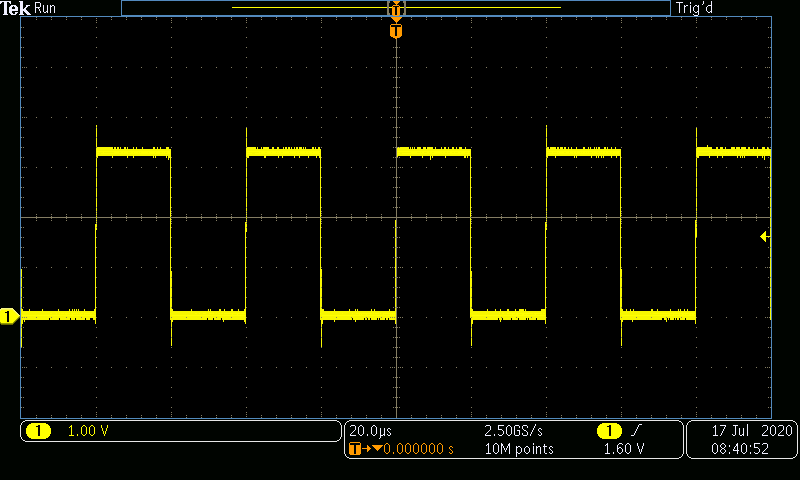
\includegraphics[width = 0.8\textwidth]{graphics/PWM_UX3_L}
\caption{Steuersignal PWM\_UX3\_L}
\label{fig:PWM_UX3_L}
\end{figure}

\newpage


\begin{figure}[h!]
\center
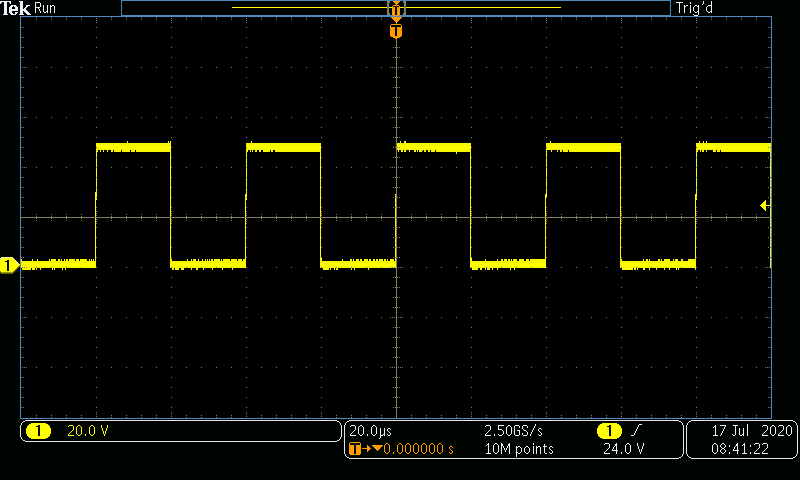
\includegraphics[width = 0.8\textwidth]{graphics/Motor_U}
\caption{Motorsignal U nach H-Brücke}
\label{fig:PWM_UX1_H}
\end{figure}

\begin{figure}[h!]
\center
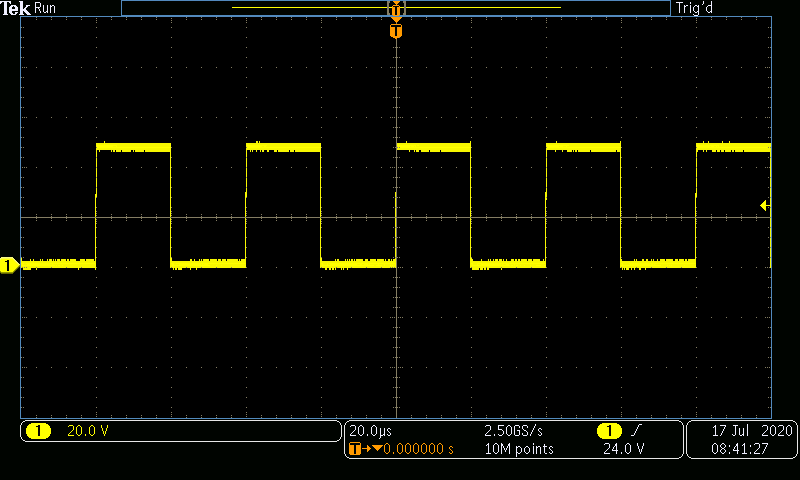
\includegraphics[width = 0.8\textwidth]{graphics/Motor_V}
\caption{Motorsignal U nach H-Brücke}
\label{fig:PWM_UX1_H}
\end{figure}

\newpage


\begin{figure}[h!]
\center
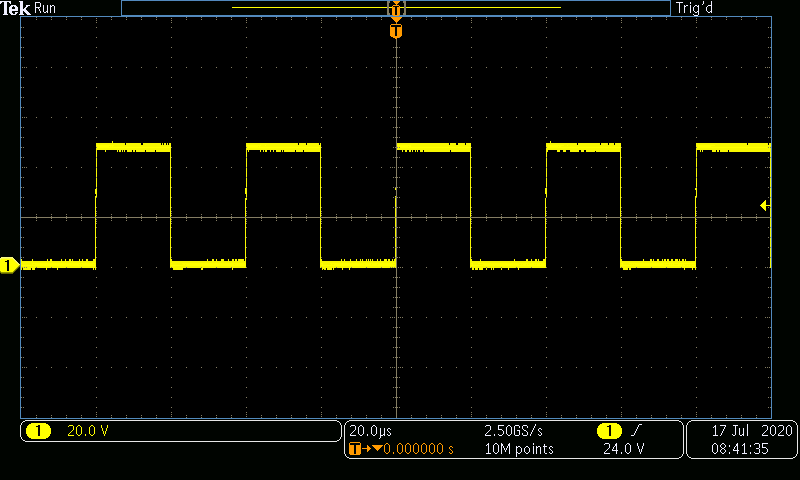
\includegraphics[width = 0.8\textwidth]{graphics/Motor_W}
\caption{Motorsignal U nach H-Brücke}
\label{fig:PWM_UX1_H}
\end{figure}


\newpage

\section{TMC6200}\label{Appendix:TMC6200}

\subsection{Standard-Schaltkreis TMC6200}

\begin{figure}[h!]
	\centering
	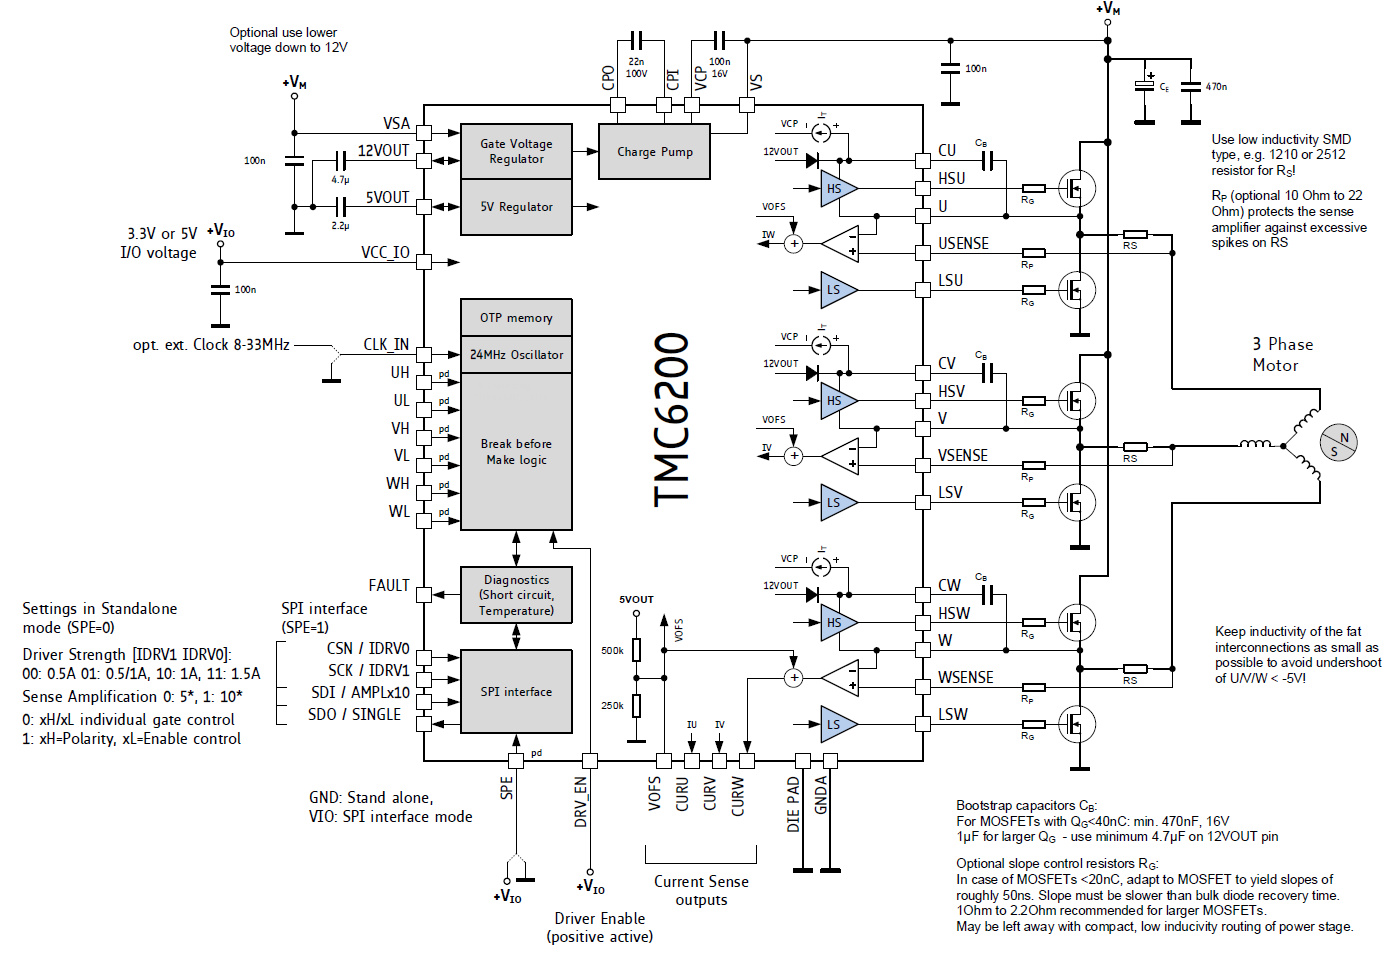
\includegraphics[width=0.8\textwidth]{graphics/Standard_Application_Cirquit_TMC6200.png}
	\caption{Standard-Anwendungs-Schaltung TMC6200.}
	\label{fig:Schaltung_TMC6200}
\end{figure}

\subsection{Blockdiagramm TMC6200}

\begin{figure}[h!]
	\centering
	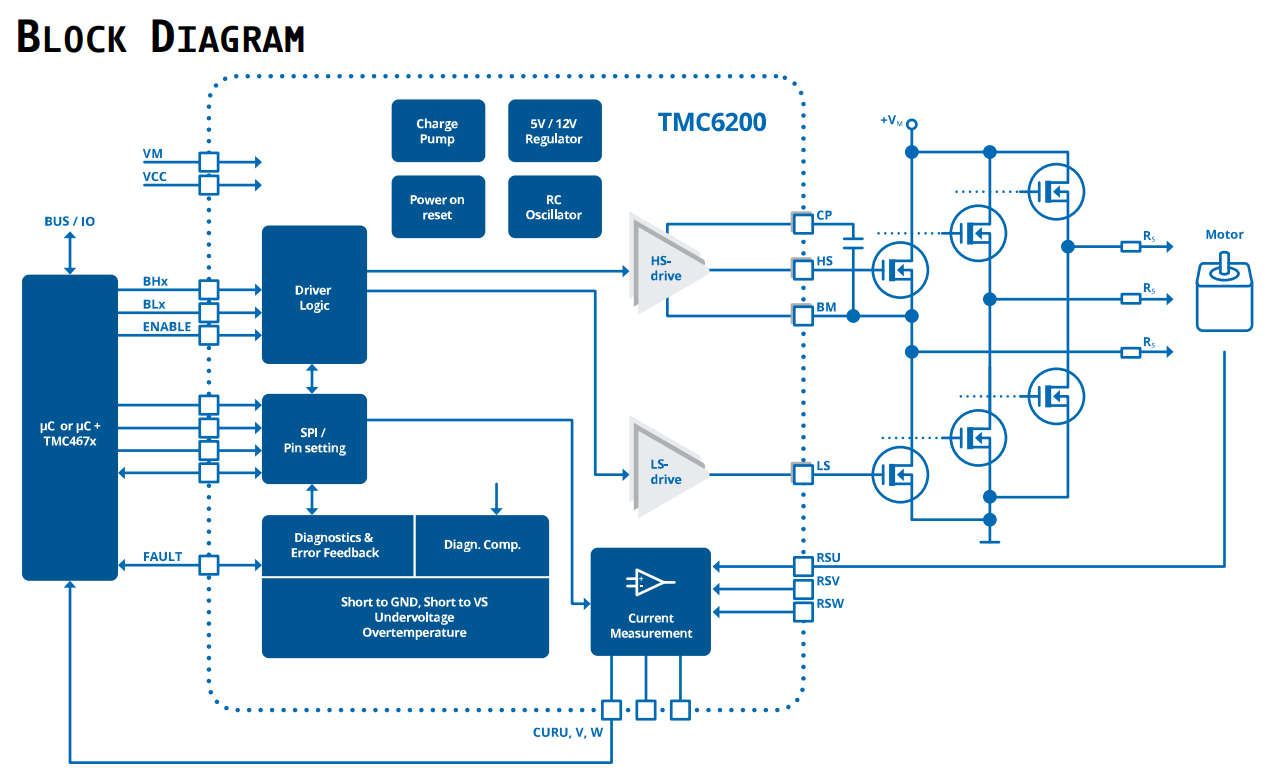
\includegraphics[width=0.8\textwidth]{graphics/Blockdiagramm_TMC6200.png}
	\caption{Blockdiagramm TMC6200.}
	\label{fig:Blockdiagramm_TMC6200}
\end{figure}

\newpage

\subsection{Verstärkungsfaktor, Strommessung, Strommesswiderstand}

\begin{figure}[h!]
	\centering
	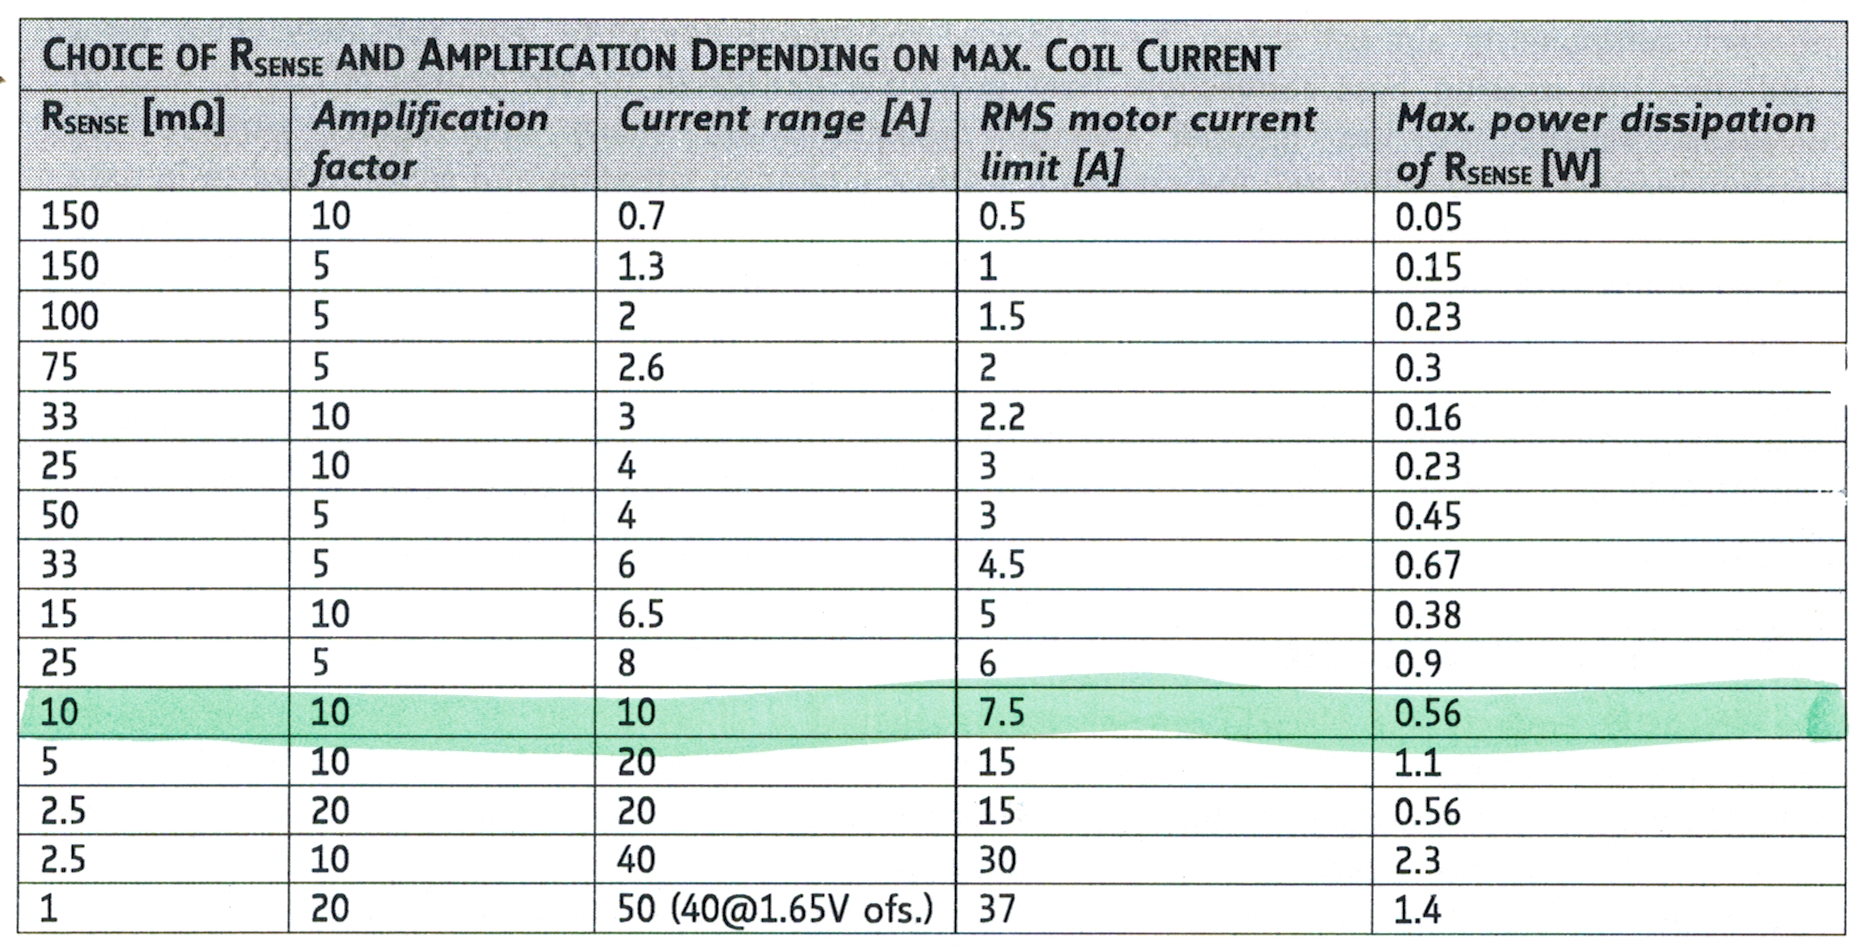
\includegraphics[width=\textwidth]{graphics/Tabelle_Shunts.png}
	\caption{Tabelle zur Bestimmung des Strommesswiderstandes aus dem Datenblatt von Trinamic.}
	\label{fig:Tabelle_Shunts}
\end{figure}

\subsection{Gate-Vorwiderstand}

\begin{figure}[h!]
	\centering
	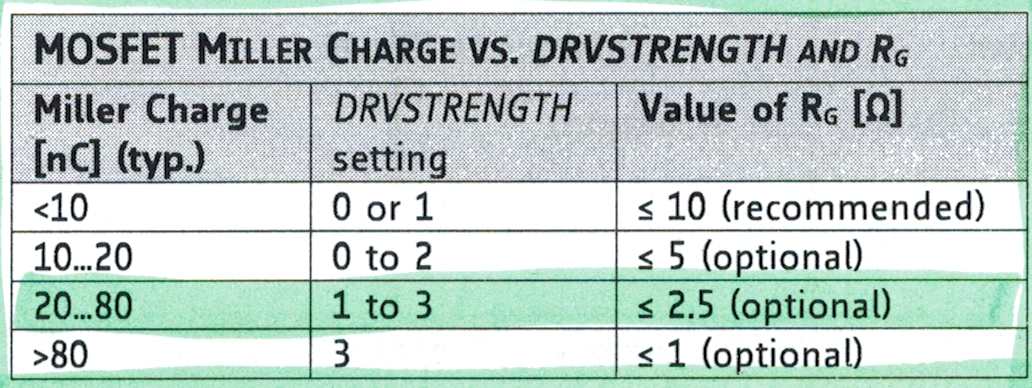
\includegraphics[width=0.5\textwidth]{graphics/Tabelle_Gatewiderstaende.png}
	\caption{Tabelle zur Bestimmung der Gatewiderstände aus dem Datenblatt von Trinamic.}
	\label{fig:Tabelle_Gatewiderstaende}
\end{figure}

\subsection{Externe Gate-Spannungsversorgung}

\begin{figure}[h!]
	\centering
	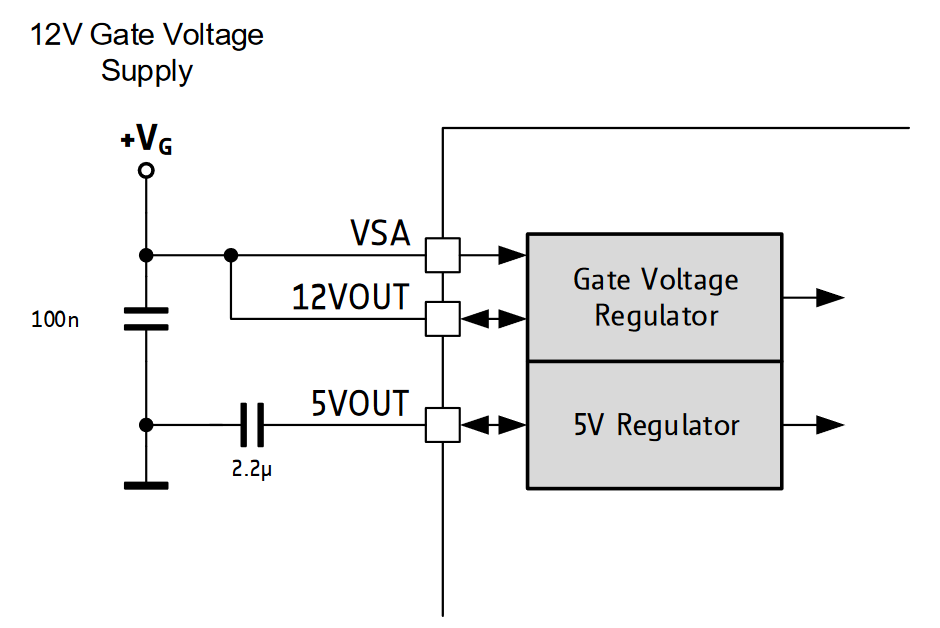
\includegraphics[width=0.5\textwidth]{graphics/Schema_Gate_Treiber_Gatespannung}
	\caption{Schema externe Gate-Spannungsversorgung.}
	\label{fig:Schema_Gate_Treiber_Gatespannung}
\end{figure}

\newpage

\section{H-Brücke}\label{Appendix:H_Bruecke}

\subsection{Referenzschema}

\begin{figure}[h!]
	\centering
	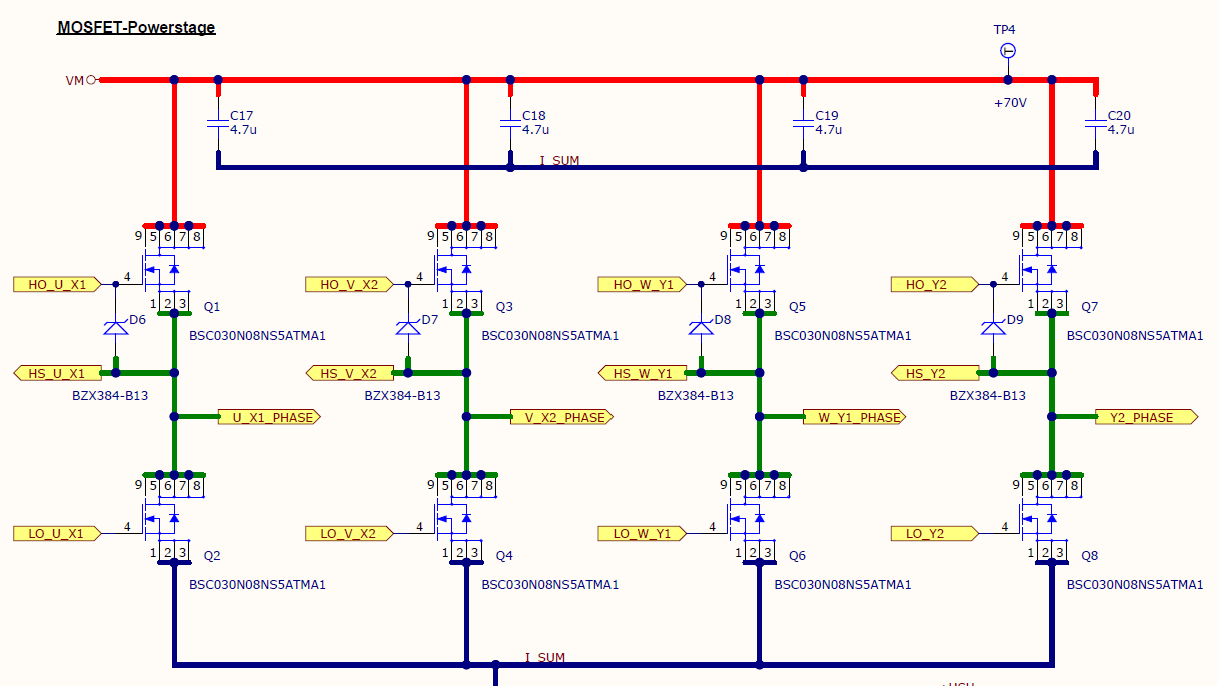
\includegraphics[width=0.7\textwidth]{graphics/Referenzschema_10A70V}
	\caption{H-Brücke.}
	\label{fig:Schema_H_Bruecke_und_BLDC_Ref}
\end{figure}

\todo{cite: Datenblatt UPS 10A70V Schema}

\section{Mikrocontroller}\label{Appendix:Mikrocontroller}

\subsection{Brown-out-Detection}\label{Appendix:Brown-out-Detection}

\begin{figure}[h!]
	\centering
	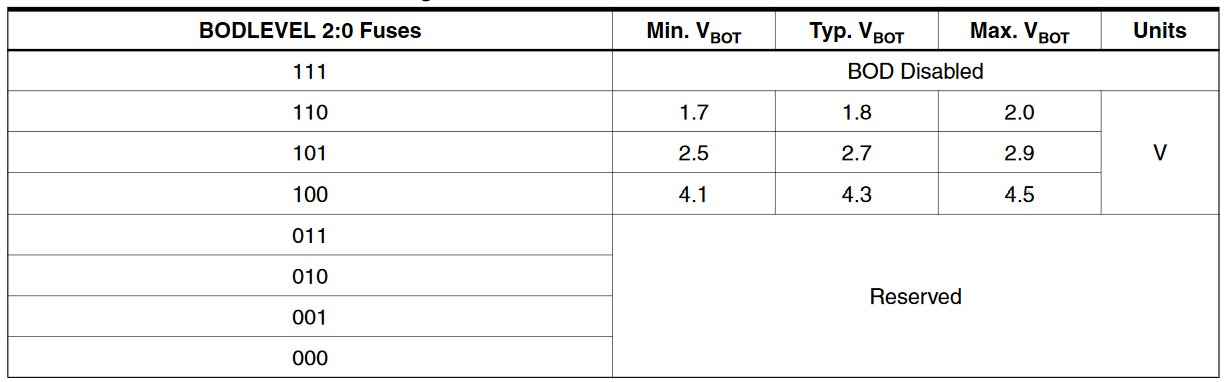
\includegraphics[width=0.7\textwidth]{graphics/Tabelle_BoD}
	\caption{Tabelle Brown-out-Detection.}
	\label{fig:Tabelle_BoD}
\end{figure}

\todo{cite: Datenblatt Atmega 2560, Seite 361}

\subsection{Full Swing Crystal Oscillator}\label{Appendix:Full_Swing _Crystal_Oscillator}

\begin{figure}[h!]
	\centering
	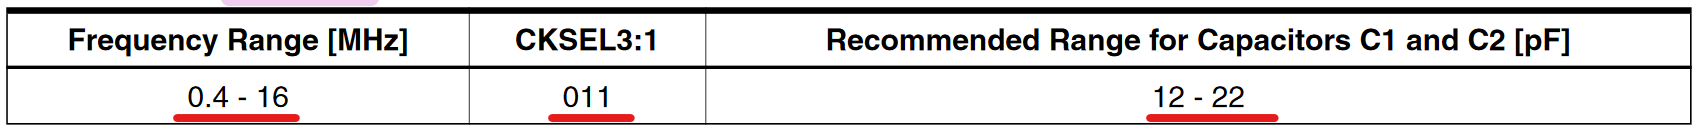
\includegraphics[width=0.7\textwidth]{graphics/Tabelle_Crystal}
	\caption{Tabelle Frequenzbereich Crystal Oszillator.}
	\label{fig:Tabelle_Crystal}
\end{figure}

\todo{cite: Datenblatt Atmega 2560, Seite 43}

\newpage

\begin{figure}[h!]
	\centering
	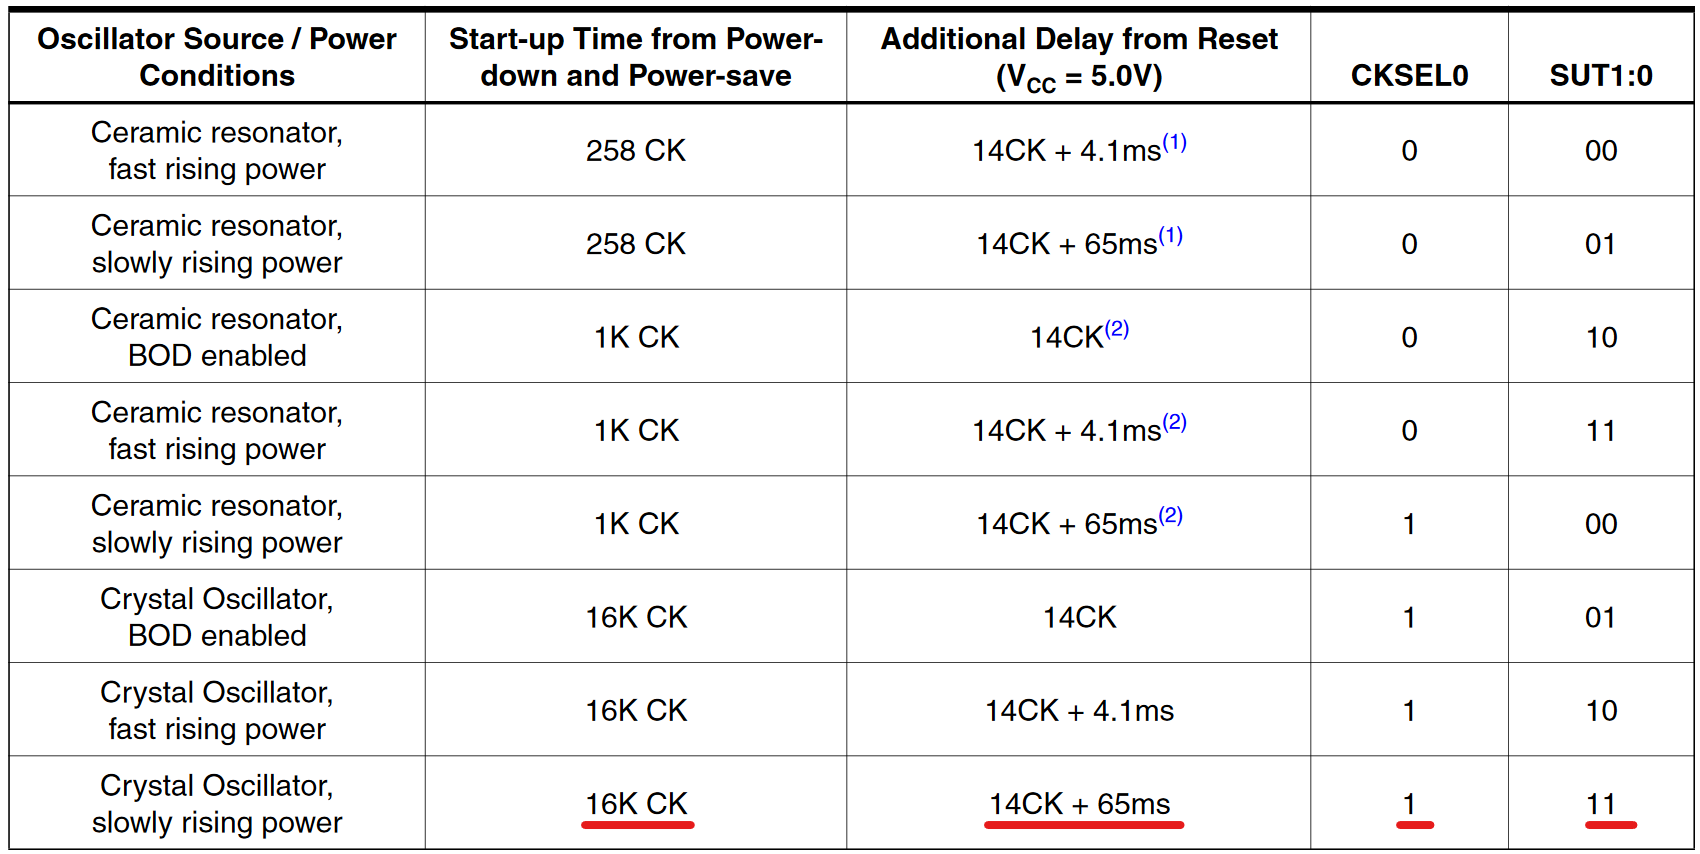
\includegraphics[width=0.7\textwidth]{graphics/Tabelle_Crystal2}
	\caption{Tabelle Aufstartzeit.}
	\label{fig:Tabelle_Crystal2}
\end{figure}

\todo{cite: Datenblatt Atmega 2560, Seite 43}

\subsection{Bootloader-Speicherplatz}\label{Appendix:Bootloader-Speicherplatz}

\begin{figure}[h!]
	\centering
	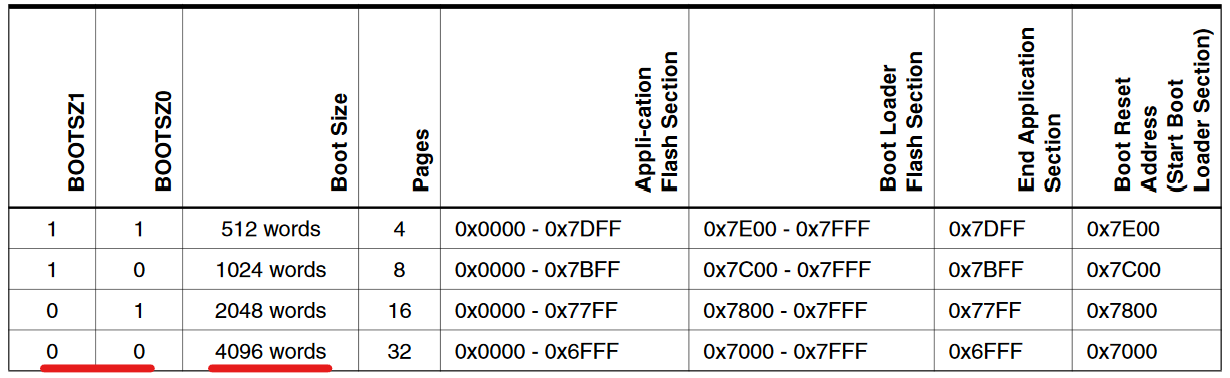
\includegraphics[width=0.7\textwidth]{graphics/Tabelle_Bootloader}
	\caption{Tabelle Bootloader Speicherplatz.}
	\label{fig:Tabelle_Bootloader}
\end{figure}

\todo{cite: Datenblatt Atmega 2560, Seite 320}

\subsection{Memory-Lock Bootloader}

\begin{figure}[h!]
	\centering
	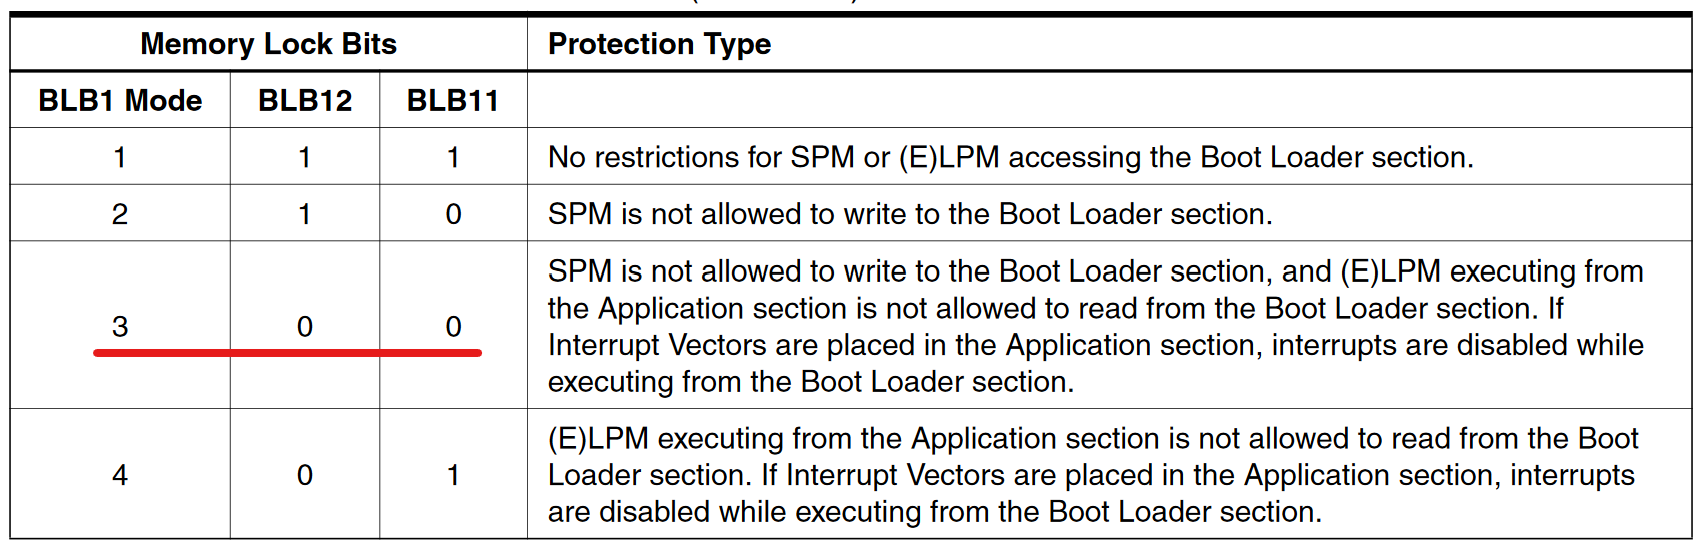
\includegraphics[width=0.7\textwidth]{graphics/Tabelle_Memory_Lock}
	\caption{Tabelle Memory Lock.}
	\label{fig:Tabelle_Memory_Lock}
\end{figure}

\todo{cite: Datenblatt Atmega 2560, Seite 326}

\newpage
\section{USB-B}\label{Appendix:USB_B}

\subsection{Geräte-Manager}

\begin{figure}[h!]
\center
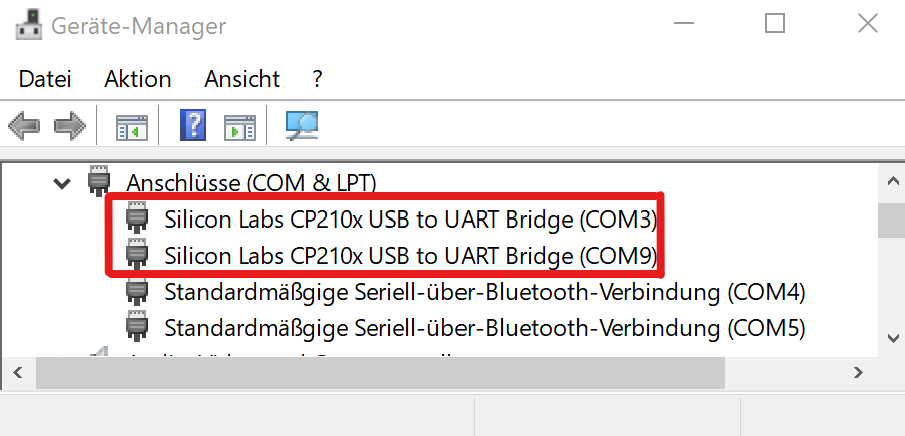
\includegraphics[width = 0.6 \textwidth]{graphics/USB_Devices_Ger_Man}
\caption{Geräte-Manager mit den aufgelisteten USB-UART-Converter (Mikrocontroller und WiFi-Modul).}
\label{fig:USB_Devices_Ger_Man}
\end{figure}

\section{Atmel Studio}\label{Appendix:Atmel_Studio}

\subsection{Fuse Bits}

\begin{figure}[h!]
	\centering
	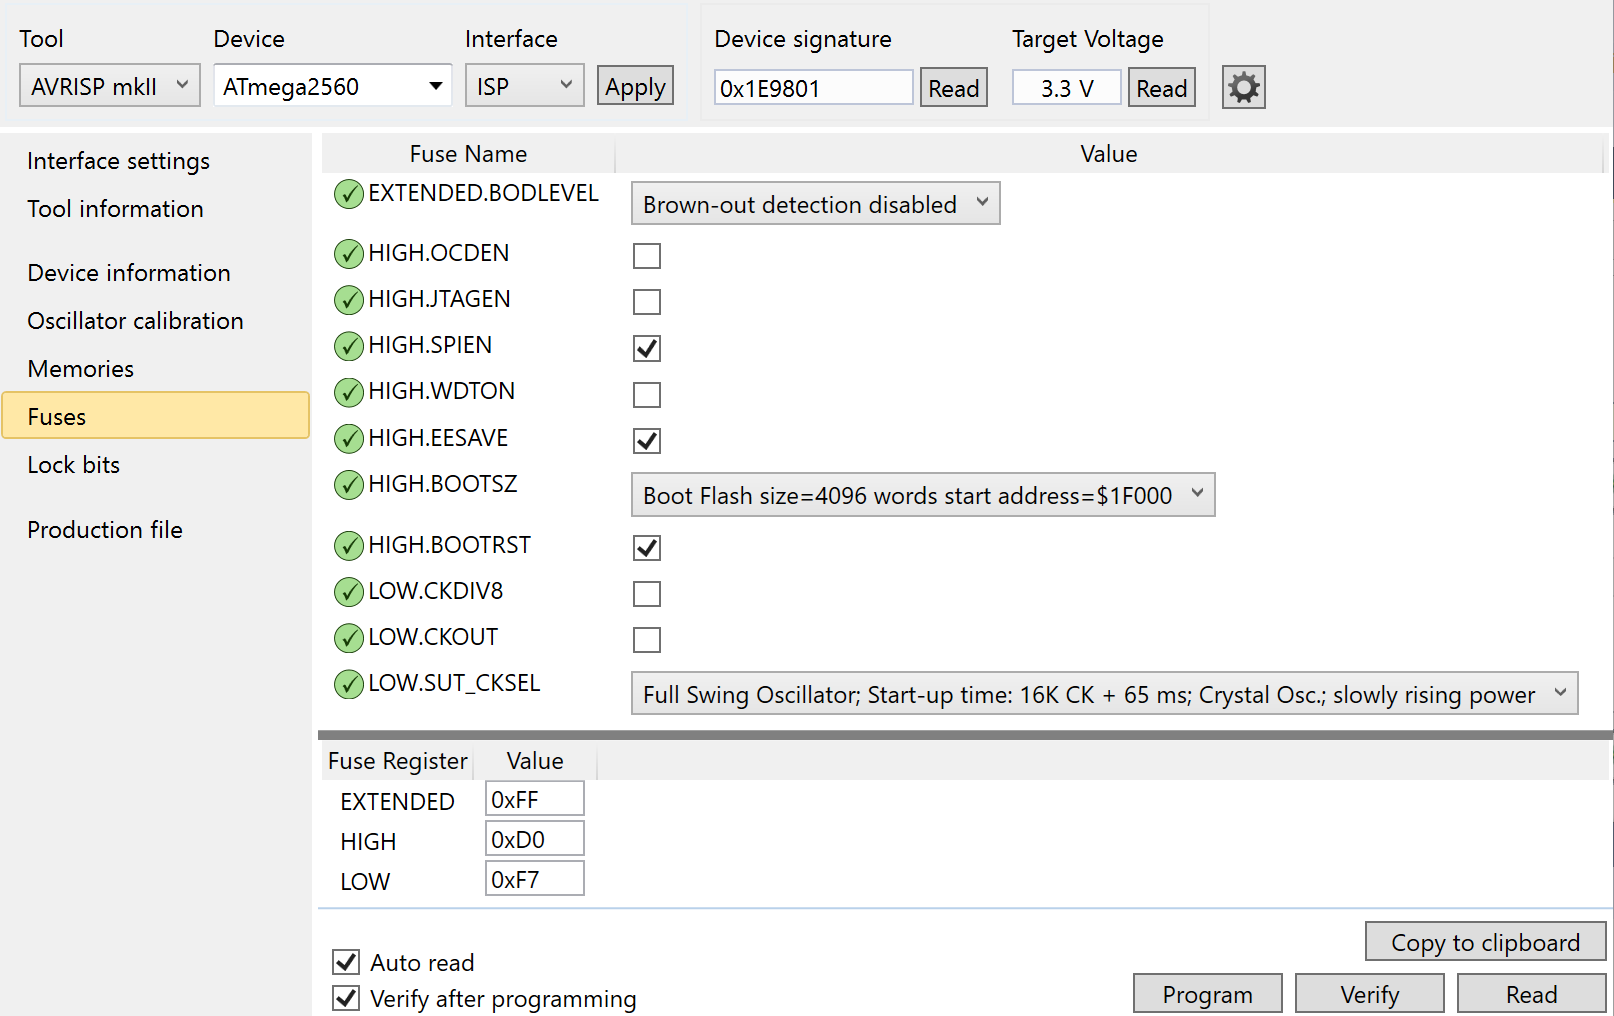
\includegraphics[width=\textwidth]{graphics/AtmelStudio_Fuses}
	\caption{Fuse-Bits Atmega2560.}
	\label{fig:AtmelStudio_Fuses}
\end{figure}

\subsection{Lock Bits}

\begin{figure}[h!]
	\centering
	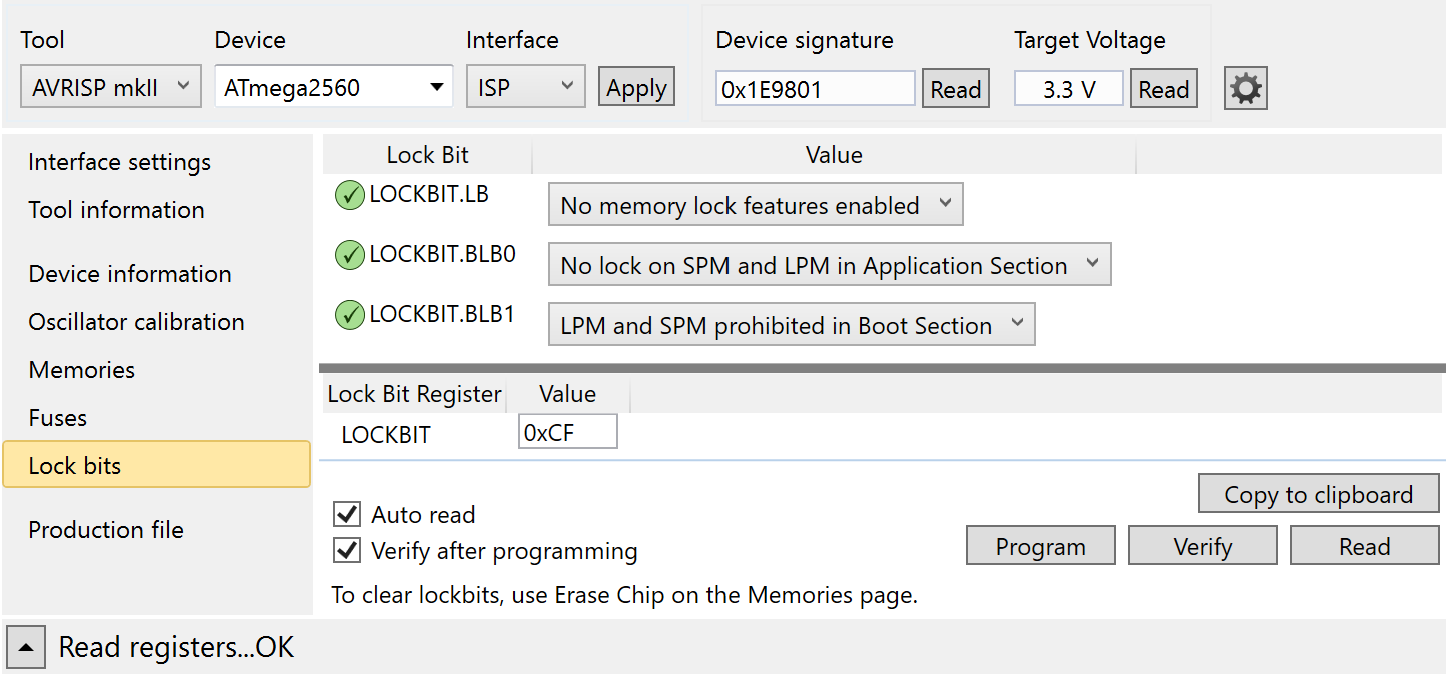
\includegraphics[width=\textwidth]{graphics/AtmelStudio_Locks}
	\caption{Lock-Bits Atmega2560.}
	\label{fig:AtmelStudio_Locks}
\end{figure}
\newpage
\subsection{Einbinden AVRdude und stk500v2 (wiring)}

\begin{figure}[h!]
	\centering
	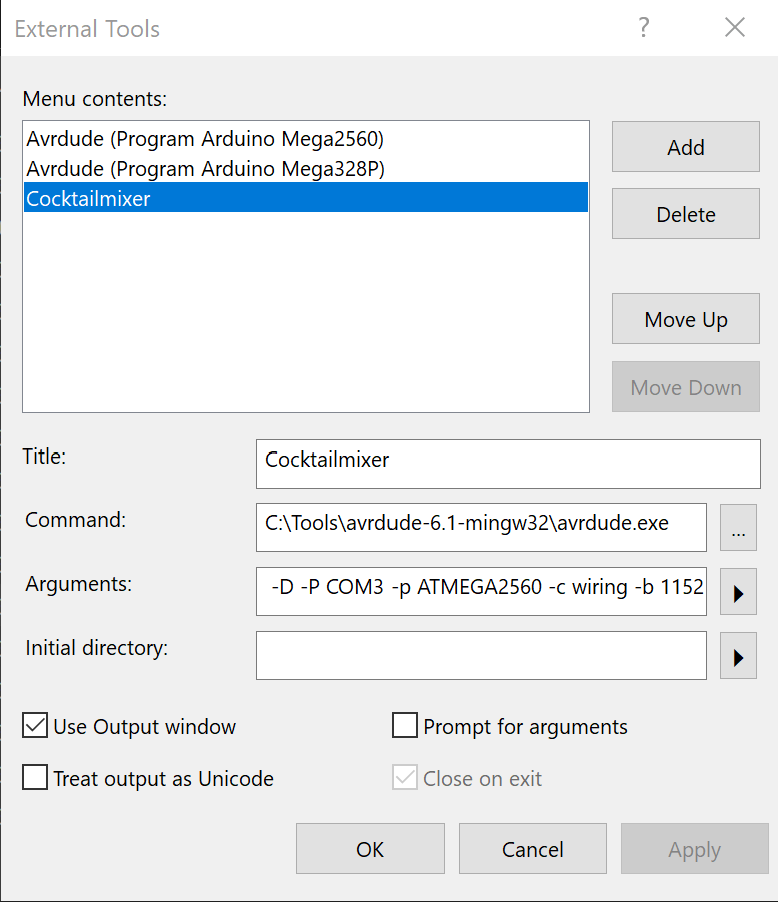
\includegraphics[width=0.5\textwidth]{graphics/AtmelStudio_External_Tools}
	\caption{External Tools Atmega2560.}
	\label{fig:AtmelStudio_Locks}
\end{figure}

\subsection{Bootloader ''Brennen''}

\begin{figure}[h!]
	\centering
	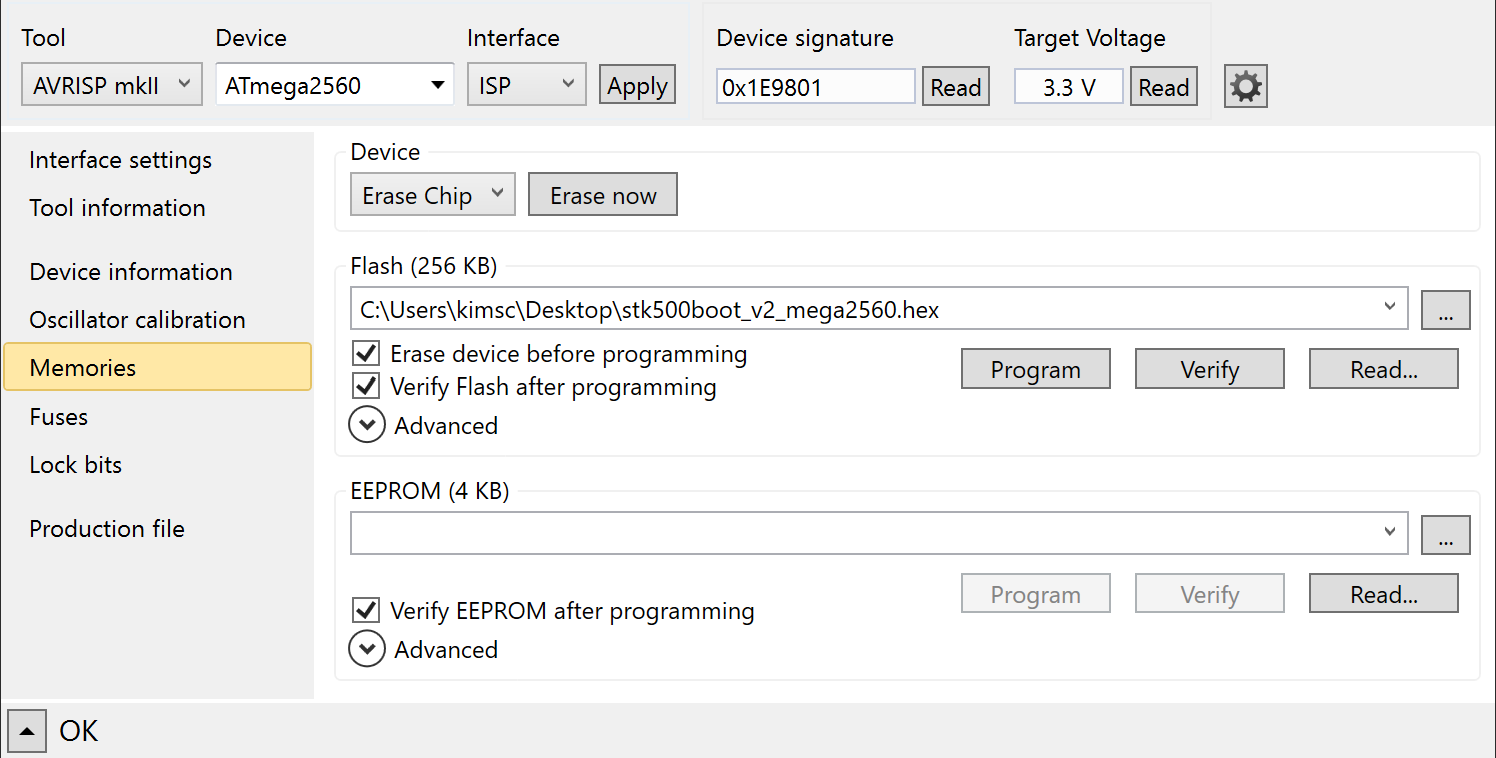
\includegraphics[width=\textwidth]{graphics/AtmelStudio_Program_Bootloader}
	\caption{Bootloader brennen.}
	\label{fig:AtmelStudio_Program_Bootloader}
\end{figure}

\end{appendix}

%%---NOTES for DEBUG---------------------------------------------------------------------
\ifdraft{%Do this only if mode=draft
%%requires \usepackage{todonotes})
\newpage
\listoftodos[\section{Todo-Notes}]
\clearpage
}
{%Do this only if mode=final
}

\end{document}
